% ||================================================================================================
% || Präambel
% ||================================================================================================

% |=================================================================================================
% | Layout
% |=================================================================================================
\documentclass[11pt,titlepage]{book}
% digital
% print
%\documentclass[12pt,titlepage]{book}
\usepackage{geometry}
\geometry{
  left=3cm,
  right=3cm,
  % print
  % bindingoffset=5mm
}

% |=================================================================================================
% | Fonts
% |=================================================================================================
\usepackage[onehalfspacing]{setspace}
\usepackage{dejavu} 
\usepackage{sectsty}
\allsectionsfont{\sffamily}
\usepackage[T1]{fontenc}
\usepackage[utf8]{inputenc} % direkte Einbgabe von Umlauten

% language stuff
\usepackage[german]{babel}

% miscellaneous
\usepackage{graphicx, subfigure}         % graphics
\graphicspath{{grafiken/}}
\usepackage{hhline}           % double lines in tables
\usepackage{amsfonts}         % real numbers etc.
\usepackage{amsmath}
\usepackage[rightcaption]{sidecap} % figure captions on the right (optional)
\usepackage{hyperref}         % for URLs
\usepackage{listings}         % for code samples
\usepackage{fancyhdr}         % for header line

\usepackage[backend=biber, style=authoryear-icomp]{biblatex}
\addbibresource{literatur.bib}
% \usepackage{natbib}
% Hier bei Bedarf die Seitenränder einstellen
\usepackage[german]{algorithm2e}
\RestyleAlgo{ruled}

\usepackage[german]{cleveref}

\usepackage{afterpage}

\newcommand\blankpage{
    \null
    \thispagestyle{empty}
    \addtocounter{page}{-1}
    \newpage
}
    
\usepackage[printonlyused]{acronym}
\usepackage{multirow, multicol, tabularx}
\usepackage{csquotes}
\usepackage{svg}

\hyphenation{Data-Frame Data-Frames}

\title{Arbeit}
\author{Alexander Martin}
\date{August 2021}
\begin{document}


\let\origdoublepage\cleardoublepage
\newcommand{\clearemptydoublepage}{%
  \clearpage
  {\pagestyle{empty}\origdoublepage}%
}

\pagestyle{empty}
\begin{titlepage}
  \begin{center}
    {\Large\bf Entwurf und Implementierung einer generischen Ingestion-Schnittstelle mit Versionierung für Data-Lake-Systeme}\\[2cm]

    {\bf Masterarbeit}\\
    zur Erlangung des Grades {\em Master of Science}\\[1cm]

    an der\\
    Hochschule Niederrhein\\
    Fachbereich Elektrotechnik und Informatik\\
    Studiengang {\em Informatik}\\[2cm]

    vorgelegt von\\
    Alexander Martin\\
    1018332\\[3cm]
    Datum: \today\\[2cm]

    Prüfer: Prof.~Dr.~rer.~nat.~Christoph Quix\\
    Zweitprüfer: Sayed Hoseini,~M.Sc.

  \end{center}
\end{titlepage}
\afterpage{\blankpage}
\include{unabhänhigkeit}
\afterpage{\blankpage}
\section*{Zusammenfassung}

Heutzutage spielen Daten eine immer wichtiger Rolle.
Durch den vermehrten Einsatz von IoT-Geräten und moderne Cloud-Speicher-Lösungen, wächst die Zahl an anfallenden Daten vielen Firmen und Forschungseinrichtungen stetig.
Mit steigenden Datenmengen und der diversen Strukturen der Daten ist deren Verwaltung ein komplexes Thema geworden.
Diese Arbeit befasst sich mit der technischen Herausforderung Daten aus verschiedensten Quellen zu Verwalten.
Als Lösung hierfür wurden Data-Lake-Systeme vorgeschlagen.
Im Kontext des HIT-Institut der Hochschule Niederrhein, wurde ein Prototyp für einen Data-Lake entwickelt.
In dieser Arbeit wird eine Schnittstelle entwickelt, über die Benutzer Daten aus unterschiedlichen Quellen in dieses System laden können.
Dabei werden Metadaten über die Datenquellen gesammelt.
Mit der Schnittstelle ist es auch möglich, die geladenen Daten zu versionieren, um weiter Verarbeitungen effizienter zu machen.

\section*{Abstract}

In todays world data play an important role.
The amount of data in comapnies and research facilities is growing due to the increasing use of IoT-devices and modern Cloud-Storage-Solutions.
With the bigger amount of data and their varying structures the data management got more complex.
This thesis takes on the technical challenge of managing data from different sources.
Data lakes are a proposed solution for this problem.
A prototype for a data lake was developed at the HIT-institute at the Hochschule Niederrhein.
This thesis devolopes an interface for users to ingest data from diffenrent sources to the system.
The interface collects metadata about the data sources.
It is also capable of saving data with versioning to make further processing more efficient.
\let\cleardoublepage\clearemptydoublepage

% Kopf- und Fußzeile
\fancyhead{} % clear all header fields
\fancyhead[RO,LE]{\leftmark}
\setlength{\headheight}{15pt}
\pagestyle{fancy}
\tableofcontents
\chapter{Einleitung}

Heutzutage spielen Daten eine immer wichtiger Rolle.
In vielen Firmen und Forschungseinrichtungen wächst die Zahl an unterschiedlichen Daten stetig.
Im \textit{Rethink Data Report 2020} \textcite{rethink_data_2020} wurde eine Studie durchgeführt, die eine Steigerung von 42\% der Menge an anfallenden Daten pro Jahr prognostiziert.
Diese Daten sind zum Beispiel durch den vermehrten Einsatz von IoT-Geräten oder ausführlicher werdende Analysen zurückzuführen.
Auch, dass es durch moderne Cloud-Speicher-Lösungen einfacher geworden ist große Datenmengen zu speichern, begünstigt diese Entwicklung.
Daten sind eine wertvolle Ressource und müssen entsprechend gut verwaltet werden.
Durch die unterschiedlichen Formate und Strukturen, zum Beispiel Datenbanktabellen, JSON-Datei oder Bilder ist die Verwaltung ein komplexes Thema.
Die Bewältigung der organisatorischen Aufgaben fällt in den Bereich Data Governance.
Diese Arbeit beschäftigt sich mit den technischen Herausforderungen Daten aus einer Vielzahl von Datenquellen zu verwalten.

In vielen Unternehmen besteht das Problem, dass Daten in sogenannten Datensilos gelagert werden.
Das bedeutet, dass für verschiedene Anwendungen oder Format isolierte Speichersysteme verwendet werden.
Dabei entsteht das Problem, dass der Überblick, welche Daten es in der gesamten Systemlandschaft gibt verloren geht.
Auch Daten, für Analysen, untereinander zu Verknüpfen wird mit zunehmender Datenmenge und Variation schwieriger.

Ein klassischer Ansatz, der die Analysen vereinfachen soll ist das Data Warehouse.
Ein Data Warehouse besteht aus verschiedenen Datamarts, in denen Daten für bestimmte Analysen abgelegt werden.
Daten werden aus den Quellsystemen geladen, mit verschiedenen Transformationen auf ein für den Datamart globales Schema gebracht und dann abgespeichert \parencite{dw}.
Dieses Vorgehen wird auch ETL (Extract Transform Load) genannt, da die Daten erst aus der Quelle extrahiert, dann transformiert und gespeichert werden und erst nach diesen Schritten für eine Analyse geladen werden können.
Bei der Transformation der Daten kann es oft passieren, dass ein Teil ihres Informationsgehalts verloren geht, da nicht alle Felder in den Datamart übernommen werden.
Außerdem wird eine Änderung an einem Schema teurer, je mehr Daten bereits integriert wurden.
Als Lösung für diese Problem wurden Data Lakes vorgeschlagen \parencite{dixon2010pentaho,datalake_03}.

\section{Data-Lake-Systeme}
\label{sec:einleitung-datalake}

Ein Data Lake ist ein System, das die Erfassung, Verfeinerung, Archivierung und Erkundung von Daten vereinfacht und verbessert \parencite{datalake_01}.
Es sollen große Datenmengen möglichst kostensparend speichern und verschiedenste Formate verarbeiten werden können \parencite{datalake_02}.
Diese System verfolgen dabei den ELT (Extract Load Transform) Ansatz.
Das Kernprinzip ist die Speicherung der Daten in ihrem Rohformat.
Die Transformation findet erst statt, nachdem die Daten für weitere Verarbeitungen geladen wurden.
Dadurch fällt der Aufwand für eine Transformation vor dem Speichern, wie bei einem Data Warehouse, weg und Daten sind schneller für weitere Verarbeitungen bereit.
Außerdem gehen dabei keine Informationen mehr verloren.

Ein Data-Lake-System basiert auf vier verschiedenen Ebenen, wie zum Beispiel in \cref{fig:datalake}.
Diese sind die Interaktion-, Transformations-, Speicher- und Ingestion-Ebene.
Über die Interaktions-Ebene kann auf die Daten im Data Lake zugegriffen und Metadaten verwaltet werden.
Die Transformations-Eben bereitet die Daten auf, nachdem diese aus der Speicher-Ebene geladen wurden.
Als letztes gibt es die Ingestion-Ebene.
Diese ist für die Integration von Daten in den Data Lake verantwortlich.
Gleichzeitig werden hier auch Metadaten aus den Daten extrahiert.
Die Umsetzung eines solchen Data  Lakes kann je nach Voraussetzungen des Einsatzbereichs variieren.

\begin{figure}
    \centering
    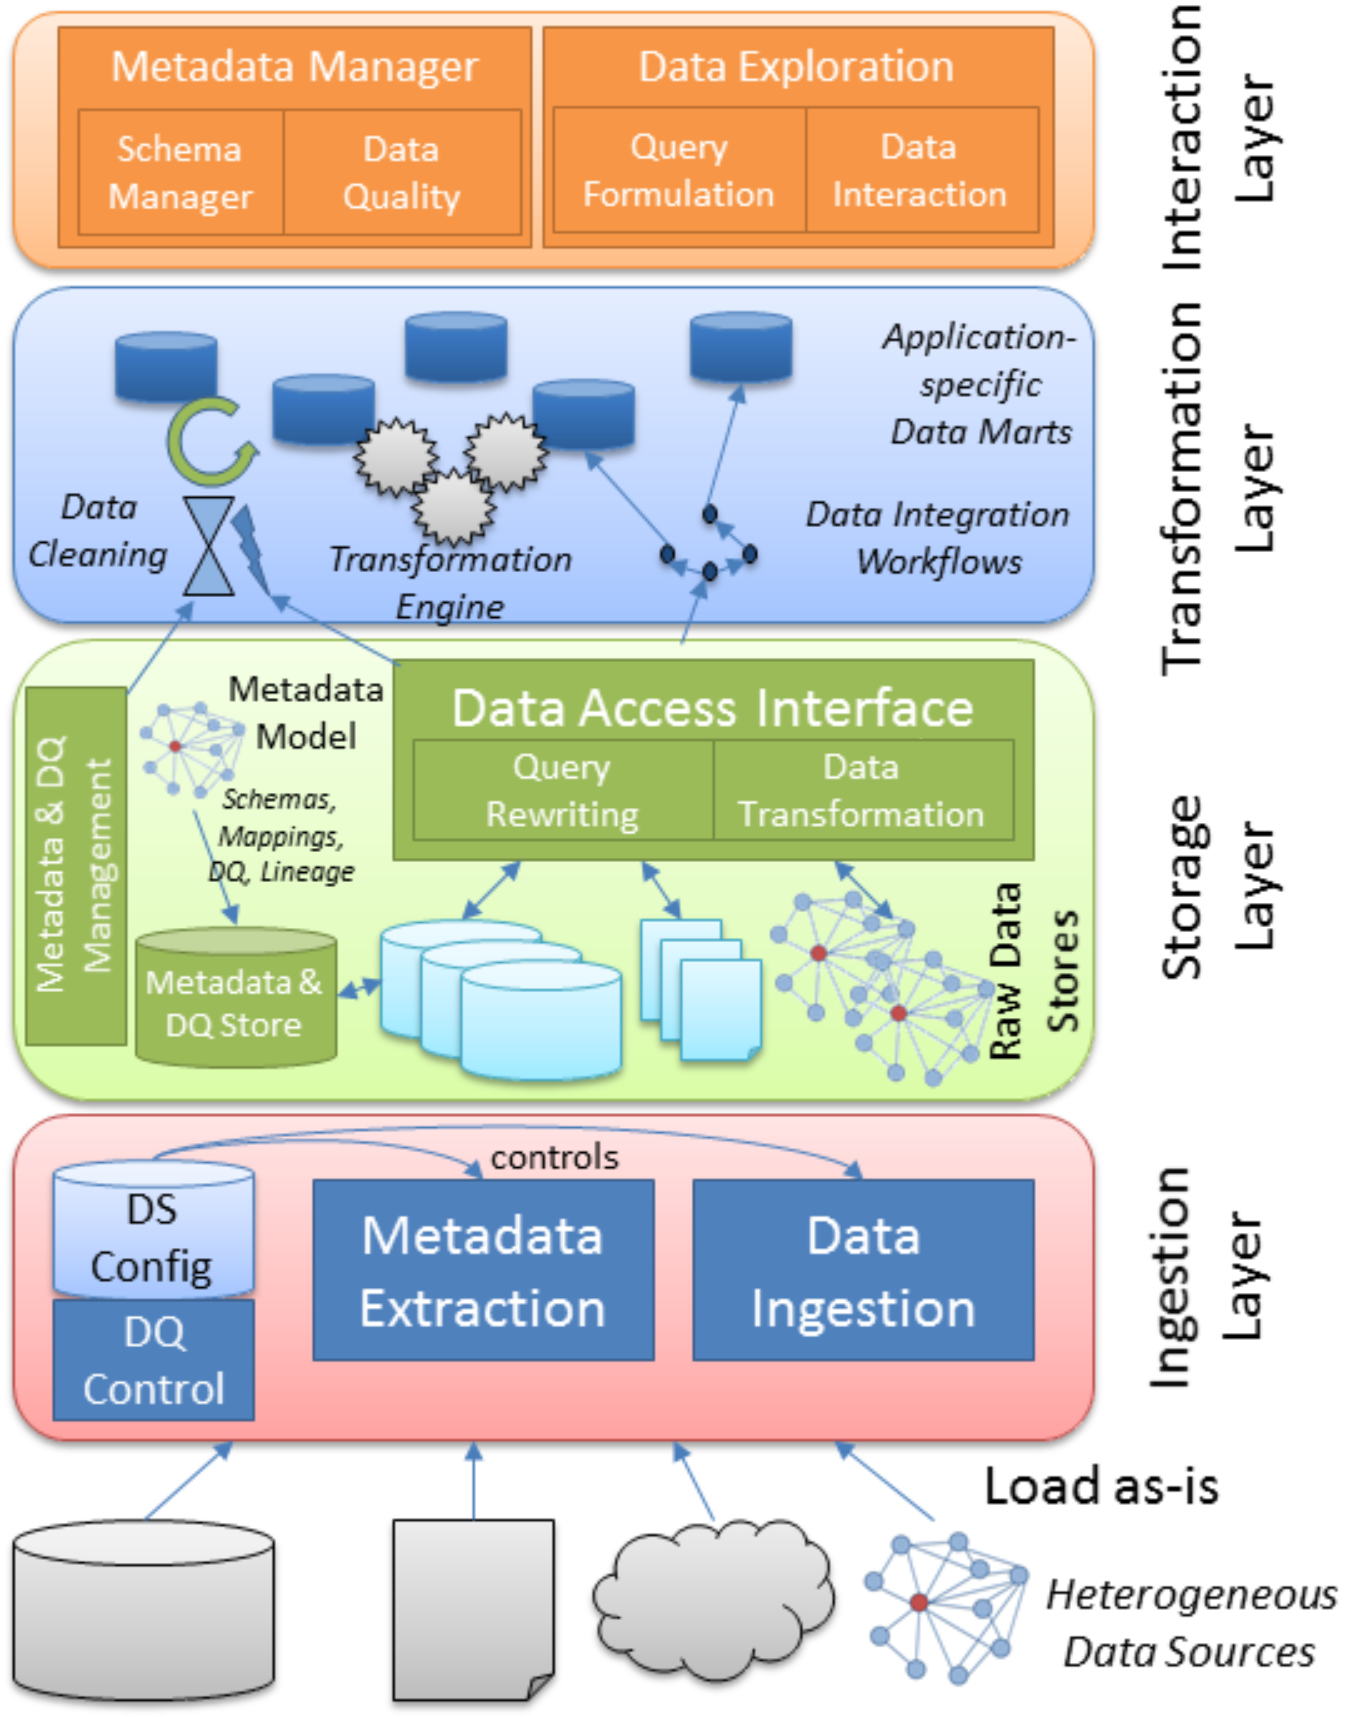
\includegraphics[width=.645\textwidth]{Grafiken/data_lake_architecture.PNG}
    \caption{Architektur eines Data Lakes \parencite{datalake_03}}
    \label{fig:datalake}
\end{figure}
\vfill

\pagebreak

\section{Motivation}
\label{sec:einleitung-motivation}

In einem Data Lake spielen die Metadaten eine zentrale Rolle.
Die Qualität der Metadaten bestimmt, wie gut Daten im Data Lake gefunden und in einen Zusammenhang gebracht werden können.
In den Metadaten können dabei sowohl Informationen über die Herkunft von Daten als auch über deren Inhalt oder Qualität stehen.

Für das HIT-Institut der Hochschule Niederrhein soll ein Data Lake entwickelt werden, der für die Verwaltung der Daten eingesetzt wird.
In diesem System sollen verschiedene Quellen zusammengebracht werden.
Dazu gehören Datenbank-Systeme, Dateien und Daten aus speziellen Software-Systemen, die über eine REST-API erreichbar sind.
Hier sollen die Daten jedoch nicht nur einmalig in das System geladen, sondern kontinuierlich aktualisiert werden.
Der einfachste Ansatz ständig den vollständigen Datensatz hinzuzufügen ist jedoch zu aufwändig und speicherintensiv.
Daher muss das Data-Lake-System eine Versionierung der Daten unterstützen und Änderungen in den Quellen erkennen können, so dass nur diese gespeichert werden.
Dies würde auch weiteren Prozessen, wie Transformation, Integration oder Analyse der Daten beschleunigen.
Diese müssten nur noch die Änderungen verarbeiten und nicht mehr den kompletten Datensatz.
Es gibt aktuell noch kein fertiges System, dass all diesen Ansprüchen genügt.

\subsection{Zielsetzung der Arbeit}
\label{sec:ziel}
In einem Masterprojekt wurde bereits ein Prototyp für ein generelles Data-Lake-System entwickelt \parencite{prototyp}.
Das bedeutet, es wurde so aufgebaut, dass der einfache Einsatz in verschiedenen Anwendungsbereichen möglich ist.
Es beinhaltet Komponenten für die Umsetzung der in \cref{fig:datalake} und durch \citeauthor{datalake_03} beschriebenen Funktionen und die dafür notwendigen Komponenten.

Mit dem Prototypen als Grundlage wird in dieser Arbeit eine Schnittstelle für die Ingestion entwickelt.
Dabei müssen drei allgemein Bedingungen erfüllt werden.
Die Schnittstelle soll unabhängig von und mit allen Datenquellen verwendet werden können.
Eine Aktualisierung der Daten soll kontinuierlich und automatisch möglich sein.
Wie vorangehen in \cref{sec:einleitung-motivation} genannt, sollen die Daten mit einer Versionierung gespeichert werden können.
Genauer betrachtet ergeben sich daraus folgende Aufgaben und Fragestellungen: \begin{itemize}
    \item Entwicklung einer Ingestion, die mit geringem spezifischen Aufwand mit allen Datenquellen kompatibel ist \begin{itemize}
        \item Wie sieht eine Ingestion aus?
        \item Wie werden Datenströme geladen?
        \item Wie werden Daten aus einer API geladen?
        \item Lässt sich daraus eine allgemeine Art der Definition ableiten, die von der Ingestion-Schnittstelle verwendet werden kann?
    \end{itemize}
    \item Die Erkennung und Speicherung von Änderungen zwischen dem aktuellen Stand im System und den Stand der Datenquelle \begin{itemize}
        \item Wie erkennt man  die Änderungen zwischen den Daten?
        \item Wann soll diese Erkennung gemacht werden?
        \item Lässt sich die Erkennung für alle Datenquellen gleich gestalten?
        \item Lässt sich die Erkennung erweiterbar gestalten, um komplexere Situationen abzubilden?
        \item Wie wird die Deltaerkennung in den Ingestion-Ablauf integriert?
    \end{itemize}
    \item Speicher und Verwalten der Versionierung von Daten \begin{itemize}
        \item Wie speichert man die Daten mit Versionierung?
        \item Wie könne Abfragen über die Datenversionen gestellt werden?
    \end{itemize}
    \item Evaluierung des Systems \begin{itemize}
        \item Anwendung des Systems mit Daten, die verschiedene Datenquellen abbilden
    \end{itemize}
\end{itemize}

\subsection{Aufbau}
Die Arbeit gliedert sich in 7 Kapitel.
Im nächsten Kapitel werden wichtige Grundlagen für die Arbeit vermittelt und verwandte Arbeiten erläutert. 
Der weitere Aufbau orientiert sich an der Vorgehensweise der Software-Entwicklung.
Zuerst werden in Kapitel 3 die Anforderungen ermittelt.
Dazu werden die Zeile für die Ingestion-Schnittstelle definiert.
Aus diesen Zielen können dann genaue Anforderungen abgeleitet werden.
Danach wird ein Entwurf für das System erstellt.
Der erste Schritt ist das Design einer Architektur.
Danach werden alle für die Umsetzung dieser Architektur benötigten Komponenten herausgearbeitet.
Kapitel 4 befasst sich mit der Umsetzung der Architektur und Komponenten.
Hier werden verwendete Techniken erläutert und begründet.
Außerdem werden wichtige Implementierungsdetails erläutert.
Auf genaue Beschreibungen der Programmierung wird verzichtet, da diese nicht bestimmend für das System sind.
In Kapitel 5 wird das System evaluiert.
Die Evaluierung teilt sich in funktionale Tests und in Benchmarks auf..
Die Arbeit schließt mit einer Zusammenfassung der wichtigsten Ergebnisse und einem Ausblick auf weitere Arbeiten
\chapter{Grundlagen und Verwandte Arbeiten}

Diese Kapitel befasst sich mit den technischen Grundlagen dieser Arbeit und verwandten Arbeiten.
Unter den technischen Grundlagen werden zunächst Rahmenwerke erklärt, die im Laufe dieser Arbeit eingesetzt werden.
% ab hier eventuell nochmal bearbeiten
Danach folgt eine genauere Erklärung des Data Lakes.
Zum Schluss wird auf das Change-Data-Capture (deutsch: Änderungserfassung) eingegangen.
Das ist nicht direkt Teil der Entwicklung in dieser Arbeit, spielt aber im Anwendungsbereich eine große Rolle.

\section{Technische Grundlagen}
\subsection{Hadoop}

Hadoop\footnote{https://hadoop.apache.org/} ist ein Projekt von Apache für die verteilte Datenverarbeitung auf einem Cluster.
Die Verarbeitung basiert auf  Map-Reduce \parencite{mapred}, einem Programmier-Modell, bei dem Daten in Form von Schlüssel-Wert-Paaren verarbeitet werden.
Grob beschrieben, besteht es aus zwei Funktionen.
Die erste ist die Map-Funktion, bei der aus Daten eine Zwischensammlung von Schlüssel-Wert-Paaren erzeugt wird.
Danach werden diese nach den Schlüsseln sortiert und die Reduce-Funktion, zum Zusammenfassen der Paare ausgeführt.
Ein Hadoop-Cluster enthält zwei wichtige Komponenten.
YARN \parencite{yarn} wird für das Ressourcen-Management benutzt.
Die zweite Komponente, das HDFS, ist ein verteiltes und fehlertolerantes Dateisystem, welches ursprünglich für Hadoop entwickelt wurde.
Für dieses Projekt ist nur das HDFS relevant und wird deswegen näher erläutert.

Das HDFS wurde entwickelt, um auf Hardware mit geringen Kosten zu laufen und große Datenmengen zu verarbeiten.
Dateien können von einem Gigabyte bis mehrere Terabyte groß sein.
Die Fehlertoleranz wird dabei durch die Möglichkeit der Replikation mit einem beliebigen Faktor gegeben.

Das Dateisystem ist ähnlich zu anderen bekannten Dateisystemen aufgebaut.
Dateien und Ordner können im Namensraum hierarchisch organisiert werden.
Es unterstützt jedoch keine Zugriffsberechtigung oder Hard- und Soft-Links.
Um einfach und effektiv kohärent zu bleiben, werden Dateien nur einmal geschrieben, können aber mehrfach gelesen werden.
Dateien werden zur Speicherung in einzelne Blöcke aufgeteilt.
Dabei sind für eine Datei alle Blöcke, bis auf den letzten, gleich groß.

\begin{figure}
    \centering
    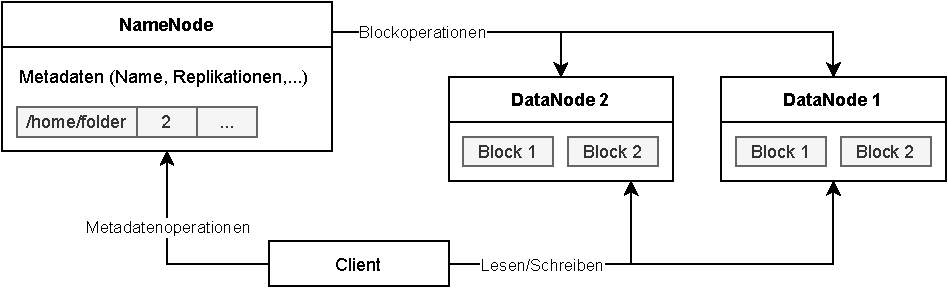
\includegraphics[width=\textwidth]{Grafiken/Grundlagen/HDFS.pdf}
    \caption[HDFS-Architektur]{HDFS-Architektur\footnotemark}
    \label{fig:hdfs-cluster}
\end{figure}
\footnotetext{Nach https://hadoop.apache.org/docs/r1.2.1/images/hdfsarchitecture.gif, Zugriff: 29.12.2021}

Ein HDFS-Cluster (\cref{fig:hdfs-cluster}) funktioniert nach dem Master-Worker-Prinzip und besteht aus einem NameNode und vielen DataNodes.
Der NameNode übernimmt die Verwaltung des Namensraums und die Verteilung der einzelnen Blöcke einer Datei.
Er reguliert dazu noch den Zugriff durch Clients und führt Operationen auf dem Dateisystem, wie das Öffnen, Schließen oder Umbenennen von Ordnern und Dateien aus.
Die DataNodes speichern die einzelnen Blöcke der Dateien.
Auf Anweisung des NameNode werden Blöcke erstellt, gelöscht oder repliziert.
Außerdem bearbeiten sie Anfragen zum Lesen und Schreiben von Dateien \parencite{hdfs}.

% Parquet
Mit Apache Parquet steht ein Format zur Verfügung, mit dem Daten im HDFS effizient gespeichert werden können.
Parquet ist ein spalten-orientiertes Speicherformat, das auch die Kompression und Kodierung der Daten unterstützt.
Über einen Algorithmus zur Zerlegung von Verschachtelung ist auch das Speichern von semistrukturierten Daten möglich \parencite{parquet}.

\subsection{Apache Spark}
\label{sec:spark}

Apache Spark ist eine Datenverabeitungs-Engine für die effiziente, verteilte Verarbeitung von Big Data.
Das Ziel bei der Entwicklung von Apache Spark war es, ein einheitliches Rahmenwerk für Big-Data-Prozesse zu schaffen,
Das Problem war, das die bis dahin verbreitetste Lösung, Hadoop, keine einheitliche Abfragesprache und kein einheitliches Datenmodell hat.
Durch Spark ist das Arbeiten mit zum Beispiel mit SQL, Datenströmen, maschinellem Lernen oder Graph-Daten möglich.
Es gibt viele Bibliotheken für die Verwendung verschiedener Datenquellen in Spark.
Durch ihre Optimierung erreichen diese ähnliche Performance wie manuell dafür implementierte Big-Data-Prozesse.
Spark kann entweder lokal auf einem Computer oder auf einem Spark-Cluster nach dem Master-Worker-Modell ausgeführt werden.

Ein Kernprinzip ist die Abstraktion der Daten in RDDs (Resilient Distributed Datasets, deutsch: Resiliente Verteilte Datensätze).
RDDs sind fehlertolerante Sammlungen von Objekten, die auf die Worker-Instanzen verteilt und parallel bearbeitet werden können.
Diese werden flüchtig im Hauptspeicher gehalten, können aber für spätere schnellere Zugriffe zwischengespeichert (persistiert) werden.
Die Erstellung und Bearbeitung von RDDs geschieht über sogenannte Transformationen.
Die Transformationen werden in einem Herkunftsgraphen gespeichert, wodurch eine Wiederherstellung bei Fehlern an jedem Punkt möglich ist.

Für die Verarbeitung von strukturierten oder semistrukturierten Daten gibt es zusätzlich die eigene Abfragesprache SparkSQL, die sich stark an SQL orientiert.
Es gibt Bibliotheken für die Sprachen Scala, Java, Python und R.
Auf den RDDs gibt es noch eine weitere Abstraktionsebene, die DataFrames.
Mit DataFrames, die eine Sammlung RDDs von Datensätzen mit einem bekannten Schema sind, kann eine API benutzt werden, bei der die Bearbeitung der Daten über Funktionsaufrufe statt SparkSQL möglich ist \parencite{spark}.

Die Interaktion mit einem Spark-Cluster kann über eine interaktive Shell oder eine in einer der unterstützen Sprachen geschriebenen Job geschehen.
Informationen über die Anwendung werden im SparkContext gespeichert.
Beim Lesen und Schreiben wird das Format der Daten angegeben.
Spark unterstützt standardmäßig einige Formate, aber durch die Konfiguration mit zusätzlichen Bibliotheken im SparkContext, kann die Unterstützung weiterer Formate hinzugefügt werden.
Von den verwendeten Bibliotheken und dem Format sind auch die Optionen abhängig, die beim Lesen und Schreiben gesetzt werden müssen.
Die Optionen sind immer Schlüssel-Wert-Paare und enthalten zum Beispiel Verbindungsinformationen zu einer Datenbank oder einen Dateispeicherort \parencite{spark-website}.

\subsection{Apache Kafka}
\label{sec:kafka}

Apache Kafka ist ein verteiltes Event-Streaming-System.
Die Vermittlung der auftretenden Events läuft in Echtzeit ab.
Kafka basiert auf dem nach dem Publish-Subscribe-Modell.
Events können von Produzenten veröffentlicht werden und Konsumenten können auf diese Events abonnieren.
Durch die Verteilung in einem Cluster kann Kafka den Ausfall einzelner Server ausgleichen.
Zusätzlich können Ströme von Events für einen beliebigen Zeitraum gespeichert werden.

Kafka besteht aus einem Cluster von Servern und verschiedenen Clients.
Es gibt zwei Arten von Servern.
Die sogenannten Broaker sind für die Verteilung und Verwaltung von Events zuständig.
Andere verwenden Server Kafka Connect\footnote{https://kafka.apache.org/documentation/\#connect} um existierende Systeme, wie zum Beispiel ein Datenbank-System, in das Kafka-Cluster zu integrieren.
Die Clients sind Anwendungen, die entweder Events produzieren oder konsumieren.

In diesem System repräsentiert ein Event den Fakt, dass etwas "`passiert"' ist und besteht aus einem Schlüssel, einem Wert, einem Zeitstempel und optionalen Metadaten.
Dabei werden die Werte nicht interpretiert sonder einfach als Byte-Block versendet und können so beliebige Struktur haben.
Events werden in sogenannte Topics unterteilt.
Es kann immer mehrere Produzenten oder Konsumenten auf einem Topic geben.
Events in einem Topic können mehrfach gelesen werden und werden nicht nach dem Konsumieren gelöscht.
Es kann aber für jedes Topic eine Dauer festgelegt werden, nach der die Events verworfen werden.
Um ein Topic fehlertolerant zu machen, kann dieses repliziert werden.

Topics werden in Partitionen über verschiedene Broker aufgeteilt, so dass das ganze System gut skalierbar wird.
Ein Produzenten kann zum Beispiel Events auf mehreren Brokern gleichzeitig veröffentlichen.
Wenn ein Event in einem Topic veröffentlicht wird, wird dieses an eine der Partitionen angehängt.
Events, die den gleichen Schlüssel haben werden immer der gleichen Partition zugeordnet und Events einer Partition kommen garantiert in der Reihenfolge des Schreibens bei dem Konsumenten der Partition an \parencite{kafka-docs}.

Konsumenten können auch in Gruppen zusammengefasst werden.
Innerhalb einer Gruppe werden Events eines Topics innerhalb der Mitglieder, die dieses Topic abonniert haben, aufgeteilt.
Diese Funktion kann zum Beispiel für den Lastausgleich verwendet werden.

\section{Data Lake}
In der Einleitung (\cref{sec:einleitung-datalake}) wurde der Data Lake als Lösung für die Probleme im Big-Data-Bereich bereits kurz beschrieben. 
In diesem Abschnitt wird noch einmal genauer auf Data-Lake-Systeme, deren Definition, Architektur und existierende Systeme eingegangen.

\subsection{Defintion eines Data Lakes}
Neben der, die in der Einleitung gegeben wird, wurde von \textcite{sawadogo2021data} eine detailliertere Definition für Data Lakes aufgestellt.
Hiernach sind Data-Lake-Systeme ein skalierbarer Speicher für Daten jeden Typs.
Die Daten werden im Rohformat gespeichert und hauptsächlich durch Datenspezialisten, wie Statistiker oder Analysten, für die Extraktion von Wissen verwendet.
Ein Data Lake hat dabei die folgenden Eigenschaften: \begin{enumerate}
    \item ein Metadaten-Katalog, um die Datenqualität sicher zu stellen,
    \item Regeln und Werkzeuge für die Data Governance,
    \item Zugänglichkeit zu den Daten für verschiedene Arten von Benutzern,
    \item die Integration von Daten jeden Typs,
    \item sowohl eine logische als auch eine physische Gliederung und
    \item die Skalierbarkeit von Speicher und Verarbeitung.
\end{enumerate}

\subsection{Architekturen für Data Lakes}
Von \textcite{inmon2016data} wird das System in sogenannten Ponds (Teiche) strukturiert.
Jeder Pond ist mit einem spezialisierten Speichersystem verknüpft und beinhaltet Daten eines bestimmten Typs.
Einige Ponds führen zudem weitere Verarbeitungen der Daten, wie Aufbereitung oder Analysen aus.
Inmon hat eine Architektur aus fünf Ponds aufgestellt (\cref{fig:datalake-ponds}).
\begin{enumerate}
    \item Daten werden im Raw Data Pond im Rohformat gespeichert und fließen von dort aus in andere Teiche.
    Dieser dient also als Eintrittspunkt in das System für neue Daten.
    Nach dem Verlassen des Teichs werden die aus diesem Daten gelöscht.
    \item Der Analog Data Pond enthält analoge Daten, meist von IoT-Geräten.
    Diese werden hier auf ein aussagekräftiges und verwaltbares Volumen reduziert und umstrukturiert.
    \item In den Application Data Pond kommen Daten, die von Software-Anwendungen erzeugt wurden.
    Diese sind häufig strukturierte Daten aus relationalen Datenbank-Systemen.
    Sie werden für Analysen integriert und aufbereitet.
    \item Der Textual Data Pond enthält unstrukturierte Daten und Prozesse, die deren Analyse erleichtern.
    \item Im Archival Data Pond werden alle Daten gespeichert, die nicht mehr aktiv verwendet, aber eventuell in der Zukunft nochmal gebraucht werden.
\end{enumerate}
\begin{figure}
    \centering
    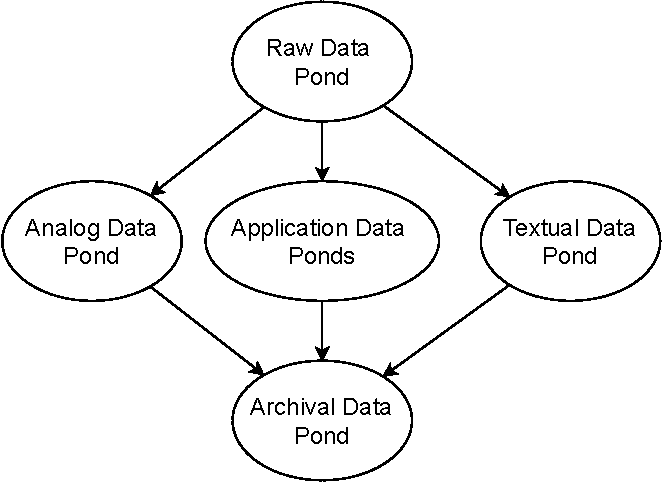
\includegraphics[width=.8\textwidth]{Grafiken/Grundlagen-Ponds.pdf}
    \caption{Ponds-Architektur eine Data Lakes nach Inmon}
    \label{fig:datalake-ponds}
\end{figure}

Ein anderer Ansatz ist die Unterteilung des Data Lakes in Zonen (\cref{fig:datalake-zones}).
Hier werden die Daten nach ihrem Verfeinerungsgrad in einer entsprechenden Zone abgelegt.
Dabei durchlaufen sie die einzelnen Zonen hintereinander.
Die Anzahl der Zonen und deren Verfeinerungsgrad ist dabei je nach Anwendung unterschiedlich \parencite{dl-zones}.

\begin{figure}
    \centering
    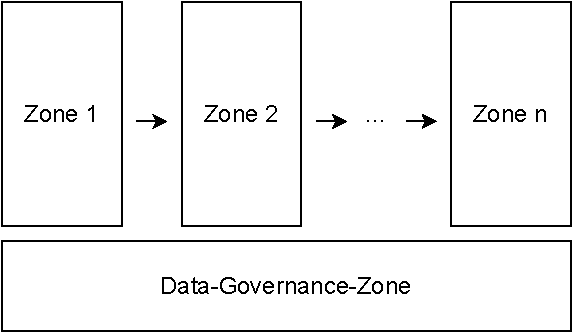
\includegraphics[width=.8\textwidth]{Grafiken/Grundlagen-Zones.pdf}
    \caption{Prinzip der Zonen-Architektur}
    \label{fig:datalake-zones}
\end{figure}

Eine speziellere Architektur ist die Lambda-Architektur, die für die verteilte Verarbeitung von Echtzeit- und Batch-Daten verwendet wird.
Eine Lambda-Architektur besteht aus drei Ebenen (Layers) \parencite{lambda-arch}. \begin{enumerate}
    \item Die Batch Layer hat zwei Aufgaben.
    Die erste Aufgabe ist das verteilte Speichern von wachsenden Daten.
    Dafür kann zum Beispiel das HDFS verwendet werden.
    Als zweite Aufgabe werden Batch Views für die verteilten Daten vorberechnet, um Anfragen schneller beantworten zu können.
    \item In der Speed Layer werden inkrementell Echtzeit-Views auf Daten verwaltet.
    Dadurch wird die Lücke gefüllt, die bei den Views in der Batch-Ebene entstehen können.
    Die Speed Layer enthält immer nur aktuelle Daten.
    Ältere Daten werden durch die Batch Layer aufgenommen.
    \item Die Serving Layer enthält Indices über alle Batch Views um Anfragen mit geringer Latenz bearbeiten zu können. Sie ist dafür verantwortlich die Views aus der Batch und der Speed Layer zusammenzuführen um Echtzeitergebnisse über alle Daten bereit zu stellen.
\end{enumerate}

Nach \textcite{sawadogo2021data} können die Architekturen von Data-Lake-System anders unterteilt werden.
Bei datenorientierten Architekturen wird der Data Lake in verschiedene Datenbereiche unterteilt.
Die funktionsorientierten Architekturen dagegen teilen das Data-Lake-System nach den Funktionen auf, die in ähnlichen Bereichen zusammengefasst werden.
Ein Beispiel ist die Architektur aus der Einleitung von \textcite{datalake_03}.
In hybriden Architekturen können auch beide Ansätze kombiniert werden.

\subsection{Existierende Data-Lake-Systeme und Rahmenwerke}
Es gibt bereits verschiedene Rahmenwerke oder Systeme für die Umsetzung eines Data Lakes.
Nachfolgend wird eine Auswahl daraus vorgestellt.

\paragraph{CoreDB} CoreDB ist ein Service, der es erlaubt über eine einzige REST-API Daten und Metadaten in einem Data Lake zu organisieren, zu indizieren und ab zu fragen. 
Es können sowohl relationale als NoSQL-Datenbanksysteme mit CoreDB verwendet werden.
Für die Suche in den Daten wird elastic\footnote{https://www.elastic.co/} verwendet.
Das Design von CoreDB unterstützt sowohl Sicherheit und Zugriffskontrolle als auch Verfolgung und Herkunft um überwachende Metadaten sammeln zu können \parencite{coredb}.

\paragraph{Azure Data Lake} In dem Cloud-Angebot von Microsoft gibt es den Azure Data Lake\footnote{https://azure.microsoft.com/de-de/solutions/data-lake/}.
Hier werden viele Funktionen, die für den Aufbau eines Data Lakes notwendig sind als Cloud-Lösung bereitgestellt.
Dazu gehören unter anderem Hadoop, Apache Spark und ein Speichersystem zum Speichern aller Daten.
Außerdem gibt es weitere Dienste zur Analyse oder Integration der Daten.

\paragraph{Kylo} Kylo\footnote{https://kylo.io/} ist ein Projekt für eine Data-Lake-Management-Plattform.
In dieser Plattform ist eine Ingestion-Komponente enthalten, die die Bereinigung und Validierung von Daten unterstützt.
Außerdem gibt es Funktionen für die Aufbereitung und Erkundung von Daten oder zur Systemüberwachung.
Zusätzlich ist Apach Nifi\footnote{https://nifi.apache.org/} zur Erstellung von Verarbeitungs-Pipelines integriert.
Die Entwicklung an Kylo wird seit über einem Jahr nicht mehr fortgeführt.

\paragraph{Hudi} Apache Hudi\footnote{https://hudi.apache.org/} ist eine Plattform, um selbst-verwaltete Data Lakes mit einer Optimierung für Datenstromverarbeitung aufzubauen.
Zu den Features von Hudi gehört zum Beispiel die Indizierung von Änderung und das Zurückgehen in den Daten zu einem bestimmten Zeitpunkt.
Hudi unterstützt sowohl inkrementelle Abfragen als auch Batch-Verarbeitung von Daten.

\paragraph{}
Bei diesen System fehlen entweder eine ausführliche Metadatenpflege oder eine Daten Versionierung, sie bilden nur einen bestimmten Teil eines Data Lakes oder sind für spezielle Anwendungsfälle.
Daher wurde bisher kein geeignetes Data-Lake-System für die Anwendung am HIT gefunden.

\subsection{Delta Lake}

Als eine Lösung für die Versionierung von Daten gibt es den Delta Lake
Delta Lake ist eine extra Speicherebene, die auf dem HDFS oder eine Objektspeicher in der Cloud, wie Amazons S3, angewendet werden kann.
Das Ziel ist es, diesen Speichern ACID-Transaktionen, schnelles Arbeiten mit Metadaten der Tabelle und eine Versionierung der Daten hinzuzufügen.
Daten werden in sogenannten Delta-Tabellen mit Metadaten und Logs gespeichert.

Eine Delta-Tabelle wird zunächst durch ein Verzeichnis im Dateisystem dargestellt.
Die tatsächlichen Daten werden in diesem Verzeichnis als Parquet-Dateien abgelegt.
Dabei können die Daten auch noch in Unterverzeichnisse aufgeteilt werden, zum Beispiel für jedes Datum ein Verzeichnis.
Neben den Datenverzeichnissen gibt es in jeder Delta-Tabelle einen Ordner für die Logs in Form von JSON Dateien mit aufsteigender Nummerierung.
Metadaten werden sowohl innerhalb der Parquet- als auch in der Log-Dateien gespeichert.

Im Delta Lake wird ein Protokoll für den Zugriff verwendet, dass es mehreren Clients ermöglicht gleichzeitig Lesen zu können, aber immer nur einem das Schreiben erlaubt.
Dabei werden beim Schreiben immer erst neue Datensätze, die zur Tabelle hinzugefügt werden sollen, in das Verzeichnis der Delta-Tabelle geschrieben.
Danach wird eine neu Log-Datei erstellt.

Beim Lesen werden die Log-Dateien als Grundlage verwendet um daraus zusammen mit den gespeicherten Daten den Zustand der Tabelle an einem bestimmten Zeitpunkt zu erzeugen.
Standardmäßig wird beim Lesen immer die aktuellste Version verwendet, man kann aber auch eine bestimmte Version angeben.
Um den Aufwand bei der Verarbeitung der Logs zu verringern wird periodisch ein Kontrollpunkt erzeugt, bei dem alle vorherigen Logs zusammengefügt und komprimiert werden.
Das bedeutet, dass zum Beispiel das Operationen die sich gegenseitig aufheben nicht gespeichert werden.
Damit reicht es aus nur den letzten Checkpoint vor der zu lesenden Version und alle darauf folgende Logs zu lesen.

Durch das Design werden keine eigenen Server für die Pflege der Delta-Tabellen benötigt.
Diese Funktionen werden von den Clients übernommen.
Der Delta Lake unterstützt sowohl die Batch-Verarbeitung von Daten als auch Datenströme und bietet volle Integration in Spark \parencite{deltalake}.


\subsection{Existierender Data-Lake-Prototyp}
In einem Masterprojekt an der Hochschule Niederrhein \parencite{prototyp} wurde ein Prototyp für ein Data-Lake-System entwickelt.
In \cref{fig:prototyp-architektur} ist ein Überblick über dessen Architektur zu sehen.
Es handelt sich hierbei um eine Client-Server-Anwendung.
Der Client besteht aus einer Web-Anwendung über die Benutzer mit dem Data-Lake-System interagieren.
Er kommuniziert mit dem Server über eine REST-API, die auch durch andere Clients verwendet werden könnte.
Die Datenverarbeitung wird über ein Spark-Cluster gelöst.
Zum Speichern der Daten stehen drei verschiedene System zu Verfügung.
Es kommen eine PostgreSQL Datenbank für strukturierte, eine MongoDB für semistrukturierte und ein HDFS für unstrukturierte Daten zum Einsatz.

\begin{figure}
    \centering
    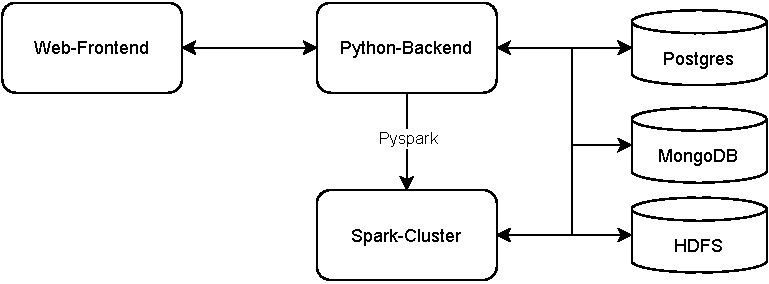
\includegraphics{Grafiken/Prototyp-Architektur.pdf}
    \caption[Architektur des Prototyp]{Architektur des Prototyp}
    \label{fig:prototyp-architektur}
\end{figure}

Die Verarbeitung der Ingestion ist im Prototyp abhängig von der Datenquelle und dem ausgewählten Zielspeicher.
In \cref{fig:prototyp-ingestion}  sind die verschiedenen Wege zu sehen.
Diese Verarbeitungsweise hat zwei Probleme, die in der neuen Ingestion gelöst werden müssen.
Dadurch, dass der Benutzer aus den verschiedenen Speichern ein Ziel auswählt, können hier leicht Probleme entstehen, falls die Datenquelle nicht mit dem Format des Speichers kompatibel ist.
Außerdem sind die Verarbeitungen der Quellen zu den Speichern fest im Code des Servers einprogrammiert.
So ist es nicht möglich während der Laufzeit neue Datenquellen zu integrieren.

\begin{figure}
    \centering
    \subfigure[Datenbank-Ingestion]{
        \label{fig:prototyp-db-ingeston}
        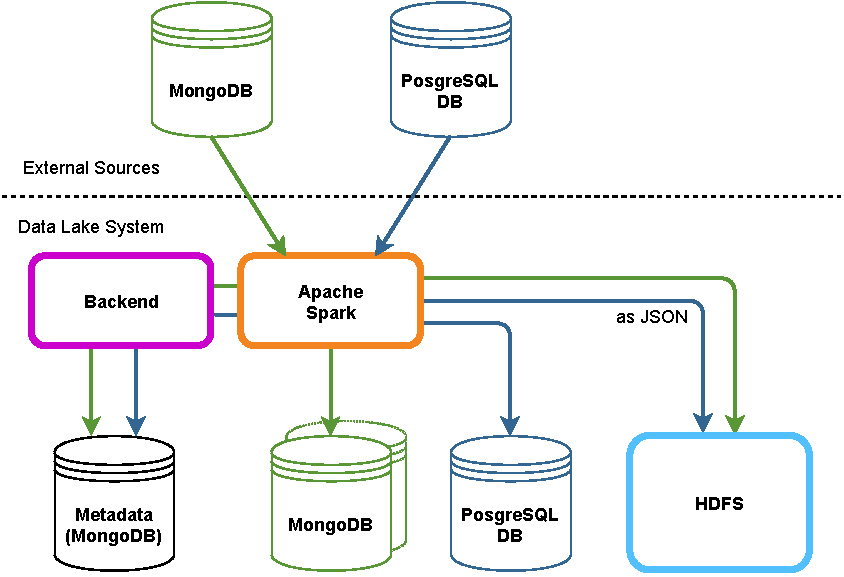
\includegraphics[width=.45\textwidth]{Grafiken/db_ingestion.pdf}
    }
    \subfigure[Datei-Ingestion]{
        \label{fig:prototyp-file-ingeston}
        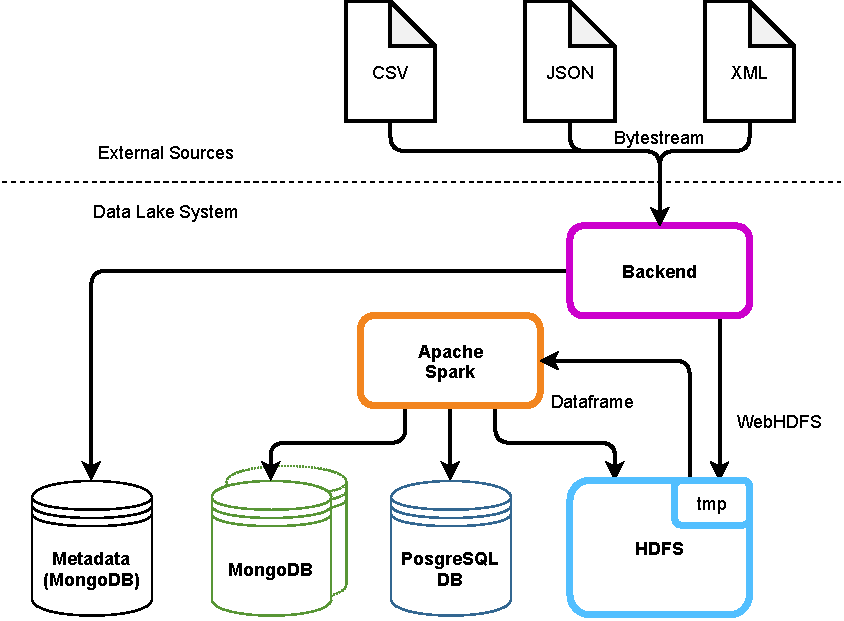
\includegraphics[width=.45\textwidth]{Grafiken/file_ingestion.pdf}
    }
    \caption[Ingestion-Verarbeitung des Prototyp]{Ingestion-Verarbeitung des Prototyp, \textcite[Quelle:][S. 3]{prototyp}}
    \label{fig:prototyp-ingestion}
\end{figure}

Im Vorlauf dieser Arbeit wurde ein Refactoring des Prototyp durchgeführt.
Dabei wurde festgestellt, dass die Erweiterung des Data-Lake-Systems um die Kompatibilität mit weiteren Datenquellen ein aufwändiger Prozess ist.
Auch durch die gewählten Speichersysteme für die geladenen Daten erschweren die Integration einer Lösung für die Versionierung der Daten.
Daher wurde beschlossen, dass eine dedizierte Ingestion-Schnittstelle für das System entwickelt werden soll.

\section{Change Data Capture}
\label{sec:cdc}

Um Änderungen an Daten in Datenquellen in das Data-Lake-System einpflegen zu können, müssen diese erst erfasst werden.
Diesen Prozess nennt man Change-Data-Capture (CDC).
Das Ziel beim CDC ist es, die Änderungen an den Daten nur an einer Stelle zu erfassen und dann an andere Systeme weiter zu geben, damit folgende Verarbeitungsschritte nur die Änderungen berücksichtigen und nicht auf den gesamten Datenbestand zurückgreifen müssen.
Dafür gibt es verschiedene Ansätze, die auf Datenbank-Triggern \parencite{boeing}, Log-Einträgen \parencite{delta-view_gen}, Zeitstempeln \parencite{delta-view_gen, boeing} oder Snapshots \parencite{cdc_in_nosql} basieren.

\subsection{Änderungserfassung Datenbank-Triggern}
Datenbank-Trigger sind Funktionen, die bei verschiedenen Aktionen auf den Daten in einer Datenbank ausgelöst werden.
Über diese Trigger lassen sich CDC-Programme realisieren, die Änderungen genau dann festhalten, wenn sie geschehen.
Ein Nachteil ist, dass die Methode nur in Systemen angewendet werden kann, die auch Trigger unterstützen.
Dafür ist es möglich alle Änderungen wie Einfügen, Aktualisieren oder Löschen von Daten zu erfassen \parencite{boeing}.

\subsection{Log-basierte Änderungserfassung}
Es gibt viele Datenspeicher-Systeme, die Logs über die Aktionen auf den Daten führen.
Diese werden zum Beispiel genutzt, um eine Wiederherstellung möglich zu machen.
Ein CDC-Programm kann diese Logs auslesen und daraus die Änderungsdaten erzeugen.
Hierdurch gibt es fast keinen zusätzlichen Aufwand für das eigentliche System.
Aber auch hier gilt, dass diese Methode davon abhängig ist ob ein System Logs erstellt und ob diese durch externe Programme abgerufen werden können \parencite{delta-view_gen}.


\subsection{Zeitstempel-basierte Änderungserfassung}
Ein weiterer Ansatz ist die Verwendung von Zeitstempeln mit den Zeitpunkten der Erstellung und letzten Änderung.
Diese Zeitstempel müssen in jedem Datensatz vorhanden sein.
Die Verantwortung dafür kann entweder bei dem Ersteller der Daten liegen oder durch das Speichersystem automatisch hinzugefügt werden.
Das CDC-Programm überprüft regelmäßig alle Zeitstempel der Einträge in den Daten.
Wenn diese zwischen dem letzten und dem aktuellen Durchlauf liegen wird die Änderung erfasst.
Hierbei werden nur kumulierte Änderungen seit dem letzten Durchlauf erfasst.
Es ist nicht möglich nachzuvollziehen, welche und wie viele Änderungen in der Zeit gemacht wurden.
Außerdem lassen sich auch mit dieser Methode kein Löschungen erfassen \parencite{delta-view_gen}.
Der Aufwand für diese Methode kann relativ hoch werden, da ohne Indices auf den Zeitstempeln immer die gesamten Daten gelesen werden müssen \parencite{boeing}.

\subsection{Snapshot-basiert Änderungserfassung}
\label{sec:snaps}
Die letzte Methode ist das Vergleichen zweier Momentaufnahmen (Snapshots) eines Datensatzes.
Dabei wird bei jedem Durchlauf zuerst ein aktueller Snapshot generiert.
Dieser wird danach mit dem des vorherigen Durchlaufs verglichen, um alle Änderungen zu erhalten.
Hierfür muss ein separater Speicherort für die Snapshots festgelegt werde.
Wie bei den Zeitstempeln ist es nicht möglich den gesamten Änderungsverlauf zwischen zwei Snapshots nachzuvollziehen.
Außerdem müssen für den Vergleich immer alle Daten geladen werden, was zu einem hohen Rechen- und Speicheraufwand führen kann \parencite{cdc_in_nosql}.
\chapter{Anforderungen}

Die Ingestion soll Daten aus unterschiedlichsten Quellen aufnehmen können.
Für die aufgenommen Daten soll das System bereits Speicher bereitstellen, die standardmäßig verwendet werden können.
Um jedoch flexibel zu bleiben muss auch die Option gegeben werden weiteres Speichersystem anzubinden.
Es reicht aus, wenn die optionale Versionierung der Daten, durch das Data-Lake-System, nur auf dem internen Speicher gegeben ist.
Änderungen am Verhalten der Ingestion in kleinerem Rahmen sollen ohne Anpassungen des Server-Codes möglich sein.

Wie bereits erwähnt, ist der Data-Lake-Prototyp eine monolithische Anwendung.
Das bedeutet, dass die gesamte Anwendung als Komplettlösung in einem Programm entwickelt und bereitgestellt wird.
Solche Ansätze sind Anfangs leichter umzusetzen, haben aber größere Nachteile in Bereichen wie Fehlertoleranz und Wartbarkeit.
Daher soll für die Ingestion-Schnittstelle der Microservice-Ansatz verfolgt werden.
Hierbei werden die Funktionalitäten und Aufgaben auf mehrere kleinere Anwendungen aufgeteilt.
Das hat den, wie von \textcite{microservices} dargestellt, mehrere Vorteile.
Die Wartung fällt bei mehreren kleinen Programmen leichter, da sie übersichtlicher und verständlicher sind.
Bei Fehlfunktionen einzelner Mircoservices fällt außerdem nicht die komplette Anwendung aus, sondern nur die Funktion, für die der Service zuständig war.
Zuletzt ist es einfacher bestimmte Aspekte der Software zu skalieren und bei Updates bleibt eine höhere Verfügbarkeit, da nur ein kleiner Teil des Systems neu gestartet werden muss.

Aus den oben genannten Zielen lassen sich jetzt genauere Anforderungen entwickeln, die die Ingestion-Schnittstelle erfüllen soll.
Dazu werden nachfolgend die einzelnen Ziele in Abschnitte aufgeteilt und die dazugehörigen Anforderungen festgehalten.
In der Evaluierung kann dann überprüft werden, ob alle Anforderung durch das Ergebnis erfüllt werden.
Die Unterkapitel sind so aufgebaut, dass erst eine genauere Erklärung für das Ziel gegeben wird und dann in einzelnen Paragraphen die Anforderungen nummeriert aufgelistet werden.

\section{Quellen- und Formatunabhänigkeit}
Es soll die Möglichkeit gegeben werden, Daten aus jeder beliebigen Quelle in das System zu integrieren.
Dazu muss die Schnittstelle sowohl in der Lage sein direkt Daten entgegen zu nehmen als auch aus anderen Systemen zu extrahieren.
Unter System wird hierbei jedoch nicht nur eine Datenbank verstanden, sonder es können unter anderem auch Dateien, APIs oder Datenströme gemeint sein.
Ebenso soll es möglich sein, den Speicher im Data-Lake-System für die Daten auszuwählen.
Da im Prototyp Apache Spark verwendet wird, ist bereits die Möglichkeit geben verschiedenste Formate zu verarbeiten.


\paragraph{ANF\_01}
\label{ANF_01}
Die Schnittstelle muss in der Lage sein Quelldaten entgegen zu nehmen, die an das Data-Lake-System gesendet werden.
Diese müssen so verwaltet werden, dass sie über Apache Spark gelesen werden können.

\paragraph{ANF\_02}
\label{ANF_02}
Da Apache Spark nicht von sich aus in der Lage ist, alle Datenformate zu verstehen, muss es möglich sein die SparkSession mit benötigten Paketen zu erweitern.

\paragraph{ANF\_03}
\label{ANF_03}
Für die Unterstützung verschiedenster Quell- und Zielsysteme verwendet Apache Spark zum Lesen und Speichern von Dateien eine Format-Parameter und Optionen.
Diese sollen komplett konfigurierbar sein um alle Systeme verwenden zu können.

\paragraph{ANF\_04}
\label{ANF_04}
Einige Funktionalitäten, wie zum Beispiel das Ausführen einer Reihenfolge von Abfragen an eine Programmierschnittstelle können nicht durch Apache Spark abgedeckt werden.
Daher soll es eine Möglichkeit geben der Ingestion-Schnittstelle eigenen Programmcode mit zu geben, der diese Funktionen abdeckt.

\section{Kontinuierliches Laden}
Da Daten sich mit der Zeit ändern, soll die Ingestion-Schnittstelle in der Lage sein, neue Daten aus einer Datenquelle, die bereits aufgenommen wurde, erneut zu laden.
Die Implementierung sollen das erneute Anstoßen, eine Zeitsteuerung oder Datenströme zulassen.

\paragraph{ANF\_05}
\label{ANF_05}
Es soll möglich sein, Datenströme in das Data-Lake-System zu integrieren und als Quelle für kontinuierliche Daten zu verwenden.

\paragraph{ANF\_06}
\label{ANF_06}
Um aktuelle Daten aus Datenquellen, die nicht über einen Datenstrom verfügen, zu integrieren, soll es eine zeitgesteuerte wiederholte Ausführung geben.

\paragraph{ANF\_07}
\label{ANF_07}
Es wird ein API-Endpunkt benötigt, über den die Ingestion für eine bestimmte Datenquelle angestoßen werden kann.
Dieser soll auch dazu verwendet werden, externe Systeme, wie eigene CDC-Lösungen anzubinden.

\paragraph{ANF\_08}
\label{ANF_08}
Eine gleichzeitige Ausführung mehrerer Ingestions auf der gleichen Datenquelle könnte leicht zu Konflikten in den Daten führen.
Daher soll sichergestellt werden, dass das System genau diesen Fall nicht zulässt.

\section{Datenversionierung}
Durch das kontinuierliche Laden von Daten, entstehen laufend neue Versionen eines Datensatzes einer Datenquelle.
Diese Veränderungen der Daten können in vielen Anwendungsfällen bei der Auswertung von Interesse sein.
Dabei gibt es zwei verschiedene Wege, diese Daten in das System ein zu pflegen.
Einmal die Verwendung von CDC-Lösungen, die bereits in den Daten die Informationen über Änderungen enthalten und zweitens kann einfach der aktuelle Stand eines Datensatzes erneut geladen werden.

\paragraph{ANF\_09}
\label{ANF_09}
Daher soll das System eine Möglichkeit bieten das Einfügen, Aktualisieren oder Löschen von Daten festzuhalten und zur Abfrage zur Verfügung zu stellen.
Außerdem sollen damit auch die Daten zu bestimmten Zeitpunkten rekonstruierbar sein.

\paragraph{ANF\_10}
\label{ANF_10}
Um für alle eingehenden Daten die Möglichkeit der Versionierung im System anbieten zu können, muss eine CDC-Implementierung eingebaut werden, die für jede Datenquelle ausgeführt werden kann.

\paragraph{ANF\_11}
\label{ANF_11}
Auch die Verwendung einer eigenen CDC-Lösung für eine Datenquelle soll unterstützt werden.
Dazu muss eine Quelle mit Änderungsdaten für eine bereits aufgenommen Datenquelle erstellt werden können.


\section{Architektur}
Wie bereits erwähnt, soll die Ingestion in einer Mircoservice-Architektur umgesetzt werden.
Außerdem wird eine Schnittstelle für die Interaktion mit dem System benötigt.
Daraus ergeben sich folgende Anforderungen, an die Architektur.

\paragraph{ANF\_12}
\label{ANF_12}
Die Interaktions-Schnittstelle mit dem System soll eine REST-API sein, die keine Konflikte mit dem aktuellen Prototypen erzeugt.

\paragraph{ANF\_13}
\label{ANF_13}
Die Aufgaben müssen klar getrennt auf die einzelnen Mircoservices aufgeteilt werden.
Die Überschneidungen zwischen den Mircoservices sollten so gering wie möglich gehalten werden.

\paragraph{ANF\_14}
\label{ANF_14}
Für die Kommunikation zwischen den Microservices soll eine einheitliche Lösung entwickelt werden.
Diese soll es auch ermöglichen neue Mircoservices einfach in die Architektur einzubringen.


\chapter{Entwurf}

Der Ingestion-Prozess ist als erster Schritt im Lebenszyklus der Daten maßgebend für deren Qualität und Aussagekraft bei der späteren Verarbeitung und Analyse \parencite{ingestion_01}.
Daher muss schon bei dem Entwurf nicht nur auf die Anforderungen Rücksicht genommen werden, sondern auch auf das fertige Data-Lake-System.

\section{Architektur}
In dieser Arbeit kann kein komplettes Data-Lake-System entworfen werden.
Es muss jedoch die Entscheidung getroffen werden, nach welcher Architektur das System aufgebaut werden soll.
Damit zuverlässig die Änderungen in einer Datenquelle erkannt werden können, dürfen die Daten, die von der Ingestion geschrieben wurden, nicht direkt verändert werden.
Hierfür ist nur die Zonen-Architektur geeignet, da Daten bei Verlassen des Raw Data Pond aus diesem glöscht werden.
Die Zonen-Architektur kann auch als eine datenorientierte Architektur bezeichnet werden.
Für die Implementierung des Data Lake soll eine Microservice-Architektur zum Einsatz kommen.
Daraus folgt, dass hier ebenfalls eine Aufteilung nach Funktionen der Komponenten notwendig ist.
Daher reicht eine pure datenorientierte Architektur des Data Lake nicht aus.
Am besten eignet sich in diesem Fall die von \textcite{sawadogo2021data} beschriebene hybride Architektur.

\subsection{Zonen-Architektur}
Von \textcite{ingestion_02} wurde eine Architektur basierend auf drei Zonen entwickelt.
\begin{enumerate}
    \item In der \emph{Drop Zone} werden alle Daten ohne weitere Verarbeitung gespeichert.
          Nur die Datenproduzenten haben Zugriff auf diese Zone und können Daten schreiben.
    \item Die \emph{Landing Zone} ist ein unveränderlicher Speicher, der Daten-Assets enthält, die jeweils zu einer Daten-Sammlung gehören. Projekte können mit den Assets aus der Landing Zone interagieren.
          Benutzer müssen lesenden Zugriff auf bestimmte Assets über einen Governance-Prozess beantragen.
    \item Projekte können in der \emph{Integration Zone} angereicherte Daten speichern.
          Diese Anreicherung kann zum Beispiel aus einer Aufarbeitung oder Umstrukturierung bestehen, die speziell für ein Projekt benötigt wird.
          Es ist außerdem möglich Daten aus der Drop Zone wieder in die Landing Zone zu laden.
\end{enumerate}
Zu diesem Zeitpunkt kann noch keine Aussage darüber getroffen werden, ob diese Architektur für die komplette Umsetzung des Data Lake geeignet ist.
Der Ansatz der Drop Zone jedoch, in der nur Datenproduzenten schreiben können, erfüllt genau die Bedingung, dass die Daten der Ingestion nicht durch andere verändert werden dürfen.
Es ist hier wichtig, dass die Daten mit denen neue Daten verglichen werden, seit der letzten Ingestion nicht verändert wurden, um genaue Aussagen über die geschehenen Änderungen in der Datenquelle treffen zu können.
Daher wird zumindest eine Zonen-Architektur mit der Drop Zone für den Entwurf übernommen.
Die Datenproduzenten, in diesem Szenario, sind alle Microservices, die für die Speicherung von Daten zuständig sind.
Die Aufteilung in Funktionen kann ebenfalls noch nicht abgeschlossen werden, da in dieser Arbeit die Ingestion-Schnittstelle nur als die erste Funktion entwickelt wird.
Weitere Funktionen werden erst im Verlauf der Entwicklung hinzugefügt.
Dabei muss aber immer mit überlegt werden, ob neben den Funktionen auch weitere Zonen in der Data-Lake-Architektur hinzugefügt werden.

\subsection{Microservice-Architektur}
\label{sec:arch}

Neben der Architektur des Data Lake muss auch eine Architektur für die Microservices entworfen werden.
Diese legt fest, welche Komponenten benötigt werden, welche Aufgaben sie bearbeiten und wie sie miteinander interagieren.
Der erste Schritt dabei ist es, trennbare Aufgaben zu identifizieren und aufzuteilen.
Der Aufbau der Microservice-Architektur kann entweder funktions- oder prozessorientiert angegangen werden.

Bei einem funktionsorientierten Aufbau wird das System in einzelne Funktionen unterteilt.
Teile dieser Unterteilung können dann einzelnen Microservices zugewiesen werden.
Für die Ingestion-Schnittstelle sind das die Funktionen zum Laden der Daten, für die Deltaberechnung und zur Speicherung der Daten.
Da diese aber ein zusammenhängender Arbeitsablauf sind, der in einem Spark-Job ausgeführt werden kann, sollten diese auch nicht auf verschiedene Microservices aufgeteilt werden.

Hier ist der prozessorientierte Ansatz besser geeignet.
Dabei werden die technischen Abläufe betrachtet, um eine Unterteilung abzuleiten.
Bei der Ingestion-Schnittstelle ergeben sich die API, das kontinuierliche Ausführen und die Ausführung der Ingestion mit Spark.
In \cref{fig:system-architektur} ist die Architektur für die Ingestion-Schnittstelle dargestellt.

Bei dem \textbf{API-Service} handelt es sich um den Service für die Interaktion mit dem Data-Lake-System.
Durch \nameref{ANF_14} ergibt sich, dass dieser ein Web-Server mit einer REST-API ist.
Es geht zwar in dieser Arbeit nur um die Ingestion, aber der API-Service sollte Schnittstellen zu allen Funktionen des Data-Lake-Systems enthalten.

Der \textbf{Ingestion-Service} ist dafür zuständig, die Datenquellen zu verarbeiten und den kompletten Prozess vom Laden bis zum Speichern der Daten in Apache Spark auszuführen.
Die Ingestion soll für eine Datenquelle nur einmal gleichzeitig, aber parallel für unterschiedliche Datenquellen ausgeführt werden können.

Bei einer zeitgesteuerten oder Datenstrom-Ingestion muss die kontinuierliche Ausführung sichergestellt werden.
Das wird durch den \textbf{Continuation-Service} übernommen.
Für alle Datenquellen muss regelmäßig geprüft werden, ob für diese gerade eine Ingestion ausgeführt wird und ausgeführt werden sollte.
Falls keine Ingestion ausgeführt wird, aber ausgeführt werden sollte, wird die Ingestion für diese Datenquelle gestartet.

Neben diesen Mircoservices wird noch ein Nachrichten-Service benötigt.
Der Nachrichten-Service stellt die Kommunikation zwischen den Microservices dar.
Hier ist es wichtig, dass es einem Sender möglich ist, Nachrichten an einen oder auch an mehrere Empfänger zu senden.
So soll sichergestellt werden, dass bestehende Microservices einfach repliziert und neue eingefügt werden können.
Für das Speichern von Daten und Metadaten wird jeweils ein Speichersystem benötigt.

\begin{figure}
    \centering
    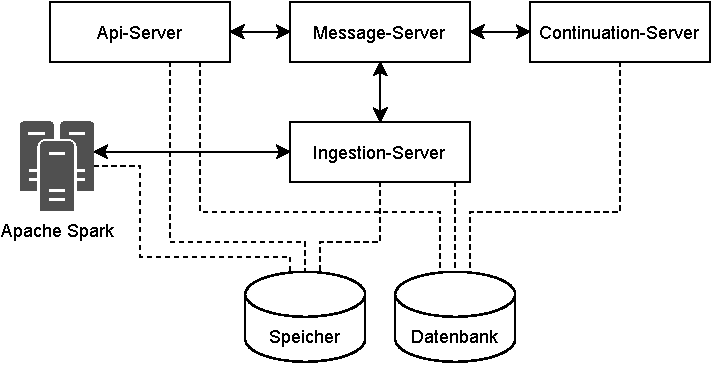
\includegraphics{Grafiken/Entwicklung-System-Architektur.pdf}
    \caption{Microservice-Architektur der Ingestion}
    \label{fig:system-architektur}
\end{figure}

\section{Plugins}

In \ref{ANF_04} wird durch ANF\_04 gefordert, dass zusätzlicher Code bei der Ingestion ausgeführt werden können soll.
Das soll durch Plugins umgesetzt werden.
Die Plugins werden jeder Datenquelle einzeln hinzugefügt und werden an verschiedenen, fest definierten Punkten der Ingestion ausgeführt. 
Da die Plugins eventuell auf Software-Bibliotheken zurückgreifen müssen, die nicht auf dem Data-Lake-System vorhanden sind, kann zusätzlich eine Liste von Abhängigkeiten der Plugins angegeben werden.

Bei der Ingestion gibt es zwei Stellen, an denen das Einbringen eines Plugins sinnvoll sein kann.
Die erste ist zum Laden der Daten als Load-Plugin.
Hier wird das standardmäßige Vorgehen der Ingestion mit dem des Plugins ersetzt.
Dadurch wird es möglich anders als nur über \textit{Apache Spark} Daten zu laden.
Ein Beispiel dafür ist die Verwendung einer REST-API als Datenquelle.
Das Plugin kann erst über mehrere Abfragen der REST-API den Datensatz abholen und diesen dann erst in eine DataFrame umwandeln.
Ein Load-Plugin muss immer eine DataFrame zurück geben, mit dem danach in der Ingestion weiter verfahren werden kann.
Damit ein DataFrame erstellt werden kann,  muss dem Plugin außerdem die entsprechende SparkSession mitgegeben werden.

Das After-Load-Plugin setzt im Gegensatz direkt nach dem Laden der Daten an.
Diesem Plugin wird das geladene DataFrame übergeben und es muss auch wieder ein DataFrame zurück geben.
Es kann genutzt werden um vor dem Speichern der Daten kleinere Anpassungen am Datensatz zu machen.
\section{Metadatenmodell}

Wie bereits erwähnt muss ein Modell erstellt werden, dass die Metadaten abbildet, die bei einer Ingestion erfasst werden (\cref{fig:datenmodell}).
Zu diesen Metadaten gehören alle Informationen über die Herkunft der Daten, also die Datenquelle und das Speicherziel.
Diese werden zum Großteil in für Spark erforderlichen Parametern widergespiegelt.
Ein weiterer Teil der Metadaten sind alle Informationen über die Ausführung einer Ingestion.

\subsection{DatasourceDefinition}

Das Metadatenmodell beschreibt eine Datenquelle und hat als zentrales Element das Konzept DatasourceDefinition.
Ein Teil des Modells besteht aus Feldern, die für Spark erforderlichen Informationen enthalten.
Dazu gehören: \begin{itemize}
    \item zusätzliche Abhängigkeiten für Spark (spark.jars.packages),
    \item das Format und Optionen für die Reader und
    \item bei benutzerdefinierten Speichersystemen das Format, die Optionen und einen Schreibmodus für die Writer.
\end{itemize}
Neben den Spark spezifischen werden noch folgende weitere Informationen erfasst: \begin{itemize}
    \item ein Name für die Datenquelle,
    \item die Id einer anderen Datenquelle, falls die aktuelle eine Update-Quelle ist,
    \item das Datum der Erstellung und letzten Änderung,
    \item den Namen der Id-Spalte in den Daten (wird später für die Deltaberechnung benötigt),
    \item den Typ, der zu lesenden Daten,
    \item eine Liste der zu laden Dateien, wenn es sich um eine Datei-Ingestion handelt,
    \item den Typ, wie die Daten geschrieben werden müssen,
    \item eine Liste mit der Zeitsteuerung für eine kontinuierliche Ingestion,
    \item eine Liste mit Plugindateien und
    \item eine Liste mit Abhängigkeiten der Plugins.
\end{itemize}

Die möglichen Lese-Typen ergeben sich aus der Betrachtung, wie die Daten in das Data-Lake-System gelangen und welche Struktur sie haben.
Bei einer Pull-Ingestion ist das System dafür verantwortlich Daten aus einer Quelle zu laden.
Dies ist zum Beispiel bei Datenbanken der Fall.
Das Gegenteil dazu ist eine Push-Ingestion, bei der die Daten direkt an den Data Lake gesendet werden.
Diese muss jedoch nochmal in zwei unterschiedliche Typen unterteilt werden.
Bei einer Stream-Ingestion, also bei Datenströmen, werden kontinuierlich neue Daten an das System gesendet.
Und bei einer File-Ingestion werden Dateien hochgeladen, die die Daten enthalten, wobei wichtig ist, dass alle Dateien das gleiche Dateiformat und je nach Typ eine ähnliche oder gleiche Struktur haben.
Die Dateien können sich in Daten- und Quelldateien unterscheiden.
Datendateien enthalten unstrukturierte Daten und werden einfach im HDFS mit abgelegt, ohne weiter verarbeitet zu werden.
Das könnten zum Beispiel Bilder oder Videos sein.
Quelldateien enthalten mindestens semistrukturierte Daten und dienen dem Zweck, in ein anderes Speicherformat, wie zum Beispiel Parquet oder eine Delta-Tabelle geschrieben zu werden.
Es ist nicht möglich, Daten direkt an die API zu senden.
Alle Push-Ingestions sollen über diese beiden Typen abgebildet werden.

Die möglichen Schreib-Typen werden aus den Speicherzielen abgeleitet.
Custom bedeutet, dass der in der DatasourceDefinition konfigurierte Speicher verwendet werden soll.
Delta ist das Speichern im internen Speicher aber mit einer Versionierung und Default ist das Speichern ohne Versionierung.

Für die Umsetzung einer unkomplizierten Versionierung der DatasourceDefinition werden alle veränderlichen Informationen in Revisionen gespeichert.
Das betrifft alle oben genannten Felder.
Die Revisionen einer DatasourceDefinition erhalten eine fortlaufende Nummer.
Die DatasourceDefinition selbst hält dann nur noch eine Liste aller Revisionen und die Nummer der aktuellen.

\subsection{IngestionEvent}

Das Modell für den Ablauf einer Ingestion ist das IngestionEvent.
Dieses enthält, wie die Revision, eine fortlaufende Nummer, ein Start- und Enddatum, den aktuellen Status indem es sich befindet, die Nummer der Revision mit der es gestartet wurde und eine Fehlernachricht, falls ein Fehler aufgetreten ist.

Das IngestionEvent kann auch zur DatasourceDefinition hinzugefügt werden.
Dafür werden Felder hinzugefügt, die alle IngestionEvents, die Nummer des letzten und die Nummer des letzten erfolgreichen IngestionEvents enthalten.

\begin{figure}
    \centering
    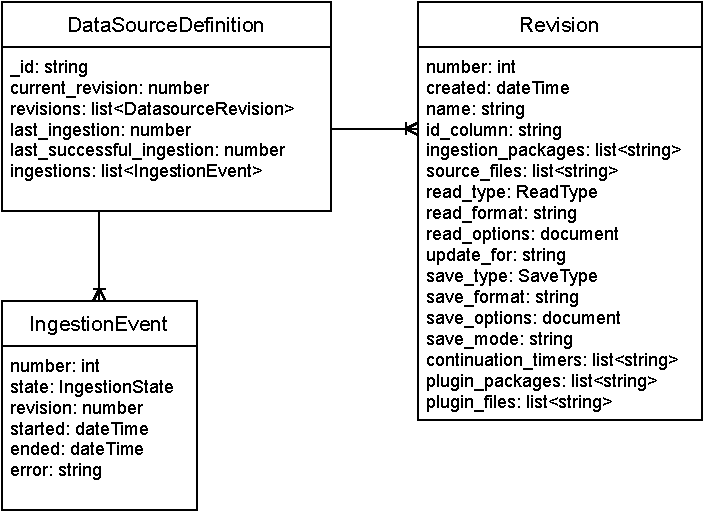
\includegraphics{Grafiken/Entwicklung-Datenmodell.pdf}
    \caption{Übersicht Metadatenmodell}
    \label{fig:datenmodell}
\end{figure}
\section{API-Service}

Für den API-Service müssen Endpunkte definiert werden.
Diese Endpunkte bilden die verschiedenen Funktionen ab, die auf der Ingestion-Schnittstelle ausgeführt werden können.
Dazu gehören die Verwaltung von Datenquellen und das Starten einer Ingestion.
Da es bereits festgelegt wurde, dass es sich um eine REST-Schnittstelle handelt, werden Endpunkte durch einen Pfad und eine HTTP-Methode definiert.
Nachfolgend werden alle Endpunkte aufgelistet.

\begin{table}[ht]
  \centering
  \begin{tabularx}{\linewidth}{lX}
    GET & /datasources \\
    \multicolumn{2}{l}{Liefert alle im System gespeicherten Datenquellen} \\
    \\
    GET & /datasources/\textless id\textgreater \\
    \multicolumn{2}{l}{Liefert die Datenquelle mit der im Pfad übergebenen Id} \\
    \\
    POST & /datasources \\
    \multicolumn{2}{l}{Bearbeitet die Daten Datenquelle mit der im Pfad übergebenen Id} \\
    \\
    PUT &  /datasources/\textless id\textgreater \\
    \multicolumn{2}{l}{Erstellt eine neue Datenquelle} \\
    \\
    GET &  /datasources/\textless id\textgreater/run \\
    \multicolumn{2}{l}{Startet eine Ingestion der Datenquelle mit der im Pfad übergebenen Id}
    
    
    
    %\hline
    %Pfad                                      & HTTP-Methode & Beschreibung                                                          \\
    %\hline \hline
    %/datasources                              & GET          & Liefert alle im System gespeicherten Datenquellen                     \\
    %\hline
    %/datasources/\textless id\textgreater     & GET          & Liefert die Datenquelle mit der im Pfad übergebenen Id                \\
    %\hline
    %/datasources                              & POST         & Erstellt eine neue Datenquelle                                        \\
    %\hline
    %/datasources/\textless id\textgreater     & PUT          & Bearbeitet die Daten Datenquelle mit der im Pfad übergebenen Id       \\
    %\hline
    %/datasources/\textless id\textgreater/run & GET          & Startet eine Ingestion der Datenquelle mit der im Pfad übergebenen Id \\
    %\hline
  \end{tabularx}
  %\caption{Endpunkte des API-Servers}
  \label{tab:enpoints}
\end{table}

Außerdem kümmert sich der API-Service um die Erstellung von Datenquellen, deren Revisionen und Ingestion-Events.
Bei Anfragen zum Starten einer Ingestion versendet der API-Server eine Nachricht, mit der Id der Datenquelle.
\section{Continuation-Service}

Für die Sicherstellung der korrekten Ausführung kontinuierlicher Ingestions, müssen regelmäßig alle Datenquellen überprüft werden.
Dabei gibt es zwei Bedingungen nach denen entscheiden wird, ob eine Ingestion werden muss.
Bei Datenströmen gilt allgemein, wenn dieser nicht läuft, dann muss die Ingestion automatisch neu gestartet werden.
Eine Ausnahme dabei ist, wenn die Verarbeitung durch den Benutzer explizit beendet wurde.

Der zweite Fall ist die Zeitsteuerung.
Für eine zeitgesteuerte kontinuierliche Ingestion werden einer Datenquelle ein oder mehrere Timer hinzugefügt.
Der Continuation-Service prüft, ob der Timer zu diesem Zeitpunkt zutrifft oder nicht.
Wenn das der Fall ist und bisher keine Ingestion auf der Datenquelle läuft, dann wird eine neue gestartet.

In Unix-Systemen gibt es bereits eine Lösung für die Notation solcher Timer.
Dort gibt es die sogenannten Cron-Jobs, mit deren Hilfe Aufgaben automatisch und regelmäßig ausgeführt werden können.
Dabei wird der Zeitpunkt der Ausführung über fünf Felder festgelegt.
Diese geben die Minute, die Stunde, den Tag des Monats, den Monat und den Tag der Woche als Zahlen an.
Als Erweiterung kann man "`*"' als Platzhalter für alle möglichen Werte verwenden, man kann mehrere Werte als mit Kommata getrennt angeben oder mit "`/x"' eine Liste in Schritten der Größe $x$ erzeugen \parencite{cron}.

Diese Notation soll auch für die Zeitsteuerung der Ingestions genutzt werden.
Als Referenz wird dabei die koordinierte Weltzeit (UTC) genommen, damit die Ausführung unabhängig vom Standort einheitlich bleibt.
Wenn eine Datenquelle mehrere Timer hat, reicht es aus, dass einer von diesen zutrifft.
\section{Ingestion-Service}
\label{sec:entw-ingestion}

Der Ingestion-Service hat die Aufgabe den Spark-Job für die Ausführung einer Ingestion zu erstellen, zu starten, zu überwachen und den Status des IngestionEvents anzupassen.
Dazu gehört das Festlegen des Ablaufs zum Laden der Daten in ein DataFrame, zur Deltaberechnung und zum Speichern.
Ein zweiter wichtiger Teil ist die Integration der Plugins in den Ingestion-Prozess.
Ebenfalls koordiniert der Ingestion-Service die parallele Ausführung von Ingestions.

Der Ingestion-Service wartet auf die Nachricht zur Ausführung einer Ingestion, mit der Id der DatasourceDefinition.
Als erstes wird geprüft, ob bereits eine Ingestion der Datenquelle aktiv ist.
Falls das nicht der Fall ist, wird ein neuer Prozess gestartet, indem die Ingestion ausgeführt wird.
Auf diese Art wird die Parallelität ermöglicht.

Der Ablauf einer Ingestion kann unabhängig vom Lese- und Schreib-Typ in einem allgemeinen Ablauf, wie in \cref{fig:ingestion-ablauf}, abgebildet werden.
Als erstes wird die Ingestion vorbereitet.
Hier werden die Plugins und deren Abhängigkeiten installiert und eine SparkSession erstellt.
Im nächsten Schritt werden die Daten aus der Quelle geladen.
Wenn es sich dabei um Änderungsdaten aus einer Update-Quelle handelt, können diese direkt in den entsprechenden Zieldatensatz eingepflegt werden.
Ist das nicht der Fall, folgt eine Entscheidung, ob Änderungsdaten berechnet werden müssen.
Es gelten die folgenden zwei Regeln: \begin{itemize}
    \item der Speicher-Typ ist Delta und
    \item es ist nicht die erste Ingestion dieser Datenquelle.
\end{itemize}
Wurden Änderungsdaten berechnet, werden diese eingepflegt.
Wurden keine berechnet, werden die Daten einfach gespeichert.
Ist das Speicherziel dabei ein Delta-Tabelle wird diese angelegt und ist es eine Parquet-Datei, dann werden die aktuellen Daten überschrieben.
Handelt es sich nicht um einen benutzerdefinierten Speicher, werden die alten Daten mit den neuen überschrieben.

\begin{figure}
    \centering
    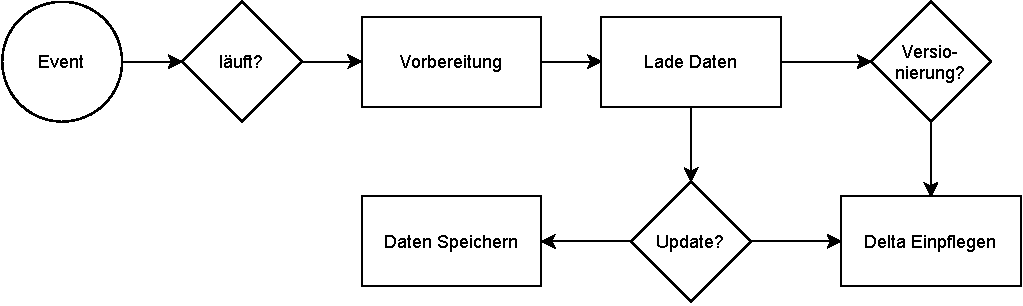
\includegraphics[width=\textwidth]{Grafiken/Entwicklung-Ingestion-Ablauf.pdf}
    \caption{Ablauf einer Ingestion}
    \label{fig:ingestion-ablauf}
\end{figure}
\chapter{Umsetzung}

Für eine Umsetzung der entwickelten Architektur ist zuerst die Frage der Techniken zu klären.
Dazu zählen die verwendete Programmiersprache, Frameworks und fertige Software.

\section{Nachrichtensystem}

Für die Übermittlung von Nachrichten zwischen verschiedenen Anwendungen gibt es sogenannte Message-Broker.
Diese koordinieren als Mittelsmann die Verteilung der Nachrichten an verschiedene Empfänger.
Das hat den Vorteil, dass der Sender unabhängig von den Empfängern wird und die Kommunikation asynchron statt finden kann \parencite{message-broker}.

Es gibt mittlerweile einige Projekte, diese Aufgabe auf verschiedene Arten lösen.
Hier wird dafür Apache Kafka verwendet, welches im Big Data Bereich weit verbreitet ist um Datenströme zu verarbeiten.
Daher macht es Sinn, dieses in das Data-Lake-System zu integrieren und darin bereit zu stellen.
Um das System dabei nicht unnötig komplex und zu groß werden zu lassen, wird daher auf einen anderen Message-Broker verzichtet.

Da Kafka ein Event-Streaming-System ist, wird ab hier nicht mehr vom Austausch von Nachtrichten, sondern von Events gesprochen.
Für diese Events müssen Topics zur Einordnung fetsgelegt werden.
Die Schlüssel sollten dabei so gewählt werden, dass Kafka auch für andere Datenströme verwendet werden kann, ohne, dass zu Konflikten kommt.
Daher werden die Topics der internen Kommunikation des Data-Lake-Systems immer mit "`dls\_\_"' als Prefix benannt werden.
Danach folgt der Bereich, den das Event betrifft, hier zum Beispiel "`ingestion"'.
An diesen Namen kann dann noch weiter Unterscheidung angehängt werden.
Für das Ausführen einer Ingestion wäre damit die Topic "`dls\_\_ingestion\_\_run"'.

Wenn mehrere Consumer in einer Gruppe für eine Topic sind, werden Events nicht an alle sondern immer nur an einen aus der Gruppe gesendet.
Dieser Mechanismus kann für den Lastausgleich an bestimmten Stellen verwendet werden.
Für die Ingestion kann so der Ingestion-Services einfach repliziert werden.
\section{Datenbank und Datenmodell}

Da das Datenmodell einer Datenquelle eine verschachtelte Struktur hat, bietet sich hier als einfachste Lösung die Verwendung einer Dokumenten-orientierten NoSQl-Datenbank an.
Das hat den Vorteil, dass diese Listen direkt in den Objekten der Datenquellen abgelegt werden können.
In relationalen Datenbanken, die Tabellen verwenden, müsste man für jedes Modell eine eigene Tabelle erstellen und die Verknüpfungen über über JOIN-Operationen auflösen.
Bei jeder Abfrage einer Datenquelle werden die verknüpften Einträge der Ingestion-Events oder Revisionen gebraucht, was somit zu einem größeren Aufwand führt.
Außerdem gibt es viele Anfragen auf die Datenquellen, da diese nicht zwischen den Mircoservices ausgetauscht werden und so nicht im Speicher vom Service verwaltet werden können.
Daher ist es effizienter die relevanten Daten direkt mit einer Abfrage laden zu können.
Hier kommt MongoDB\footnote{https://www.mongodb.com/} als Datenbank zum Einsatz.
MongoDB kann frei verwendet werden und bei bei größeren Datenmengen verteilt eingesetzt werden.

\section{Datenspeicher}

Für das Speichern von Daten mit einer Versionierung ist Delta Lake eine gut gepflegte und in Spark integrierte Lösung.
Neben den versionierten müssen auch Daten mit und ohne Struktur gespeichert werden.
Für strukturierte und semistrukturierte Daten kommt das Parquet-Format zum Einsatz.
Unstrukturierte Daten werden im ursprünglichen Format im HDFS abgelegt.

Als Speicher wird das HDFS verwendet.
In diesem können sowohl die Delta Tabellen als auch andere Parquet-, Quell- und Plugin-Dateien abgelegt werden.
Alle Microservices haben über die WebHDFS-Schnittstelle Zugriff auf die Daten.
Im HDFS wird eine Verzeichnisstruktur (\cref{fig:hdfs-folder}) für alle Daten des Data Lakes angelegt.
Diese geht von dem Ordner "`datalake"' aus, der im Root-Verzeichnis des HDFS angelegt wird.
In diesem Ordner werden die Unterordner
\begin{itemize}
    \item "`sources"' für Quell-Dateien,
    \item "`plugins"' für Plugin-Dateien und
    \item "`data"' für die Ablage von geladenen Daten erstellt.
\end{itemize}

In den Ordnern "`sources"' und "`plugins"' werden dann für jede Datenquelle Ordner mit deren Id angelegt, in denen die hochgeladenen Dateien abgelegt werden.

Für die geladenen Daten werden die Ordner \begin{itemize}
    \item "`structured"' für semi-/strukturierte Daten ohne Versionierung,
    \item "`unstructured"' für unstrukturierte Daten und 
    \item "`delta"' für semi-/strukturierte Daten mit Versionierung.
\end{itemize}
innerhalb des Ordners "`data"' angelegt.
Diese unterteilen sich dann ebenfalls wieder in Ordner für jede Datenquelle mit der Id als Name.

\begin{figure}
    \centering
    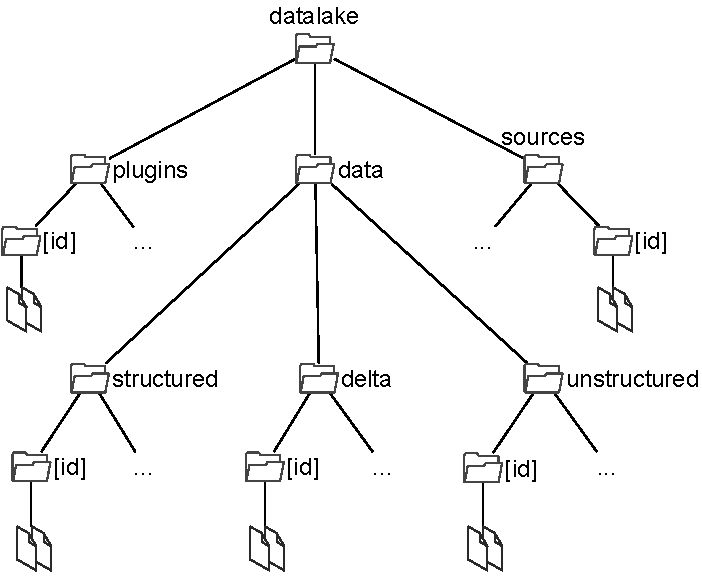
\includegraphics[width=.6\textwidth]{Grafiken/Umsetzung-Verzeichnisse.pdf}
    \caption{HDFS Verzeichnisstruktur}
    \label{fig:hdfs-folder}
\end{figure}
\section{API-Service}

Bei HTTP-Anfragen können Inhalte in der Anfrage als verschiedene Typen übergeben werden.
Hier wird der Typ \verb|mutltipart/forma-data| verwendet.
Bei diesem Typ können sowohl Text als auch Dateien übertragen werden.
Jeder Text oder jede Datei werden dabei als Wert betrachtet und müssen einen Schlüssel vergeben bekommen.
Das heißt, dass alle Informationen als Schlüssel-Wert-Paar an den API-Service gesendet werden.
Die Schlüssel, die verwendet werden sollen, werden wie folgt vergeben.
Die DatasourceDefinition bekommt den Schlüssel "`datasource-definition"'.
Der Wert dahinter kann entweder eine JSON-Datei oder ein JSON-Text sein.
Die Schlüssel der hochgeladenen Dateien sind frei wählbar.

Die DatasourceDefinition besteht zu Teilen aus Feldern, die automatisch durch die Services gefüllt werden.
Daher wird ein weiteres Datenmodell für die Eingabe von Informationen bei der REST-API benötigt.
Dafür wird die DatasourceDefinitionInput (\cref{fig:datasource-definition-input}) verwendet.
In diesem Modell befinden sich alle Felder, die durch den Benutzer befüllt werden können.
Aus den Daten dieses Modells erstellt der API-Service dann die Revisionen für die DatasourceDefinition.

\begin{figure}
    \centering
    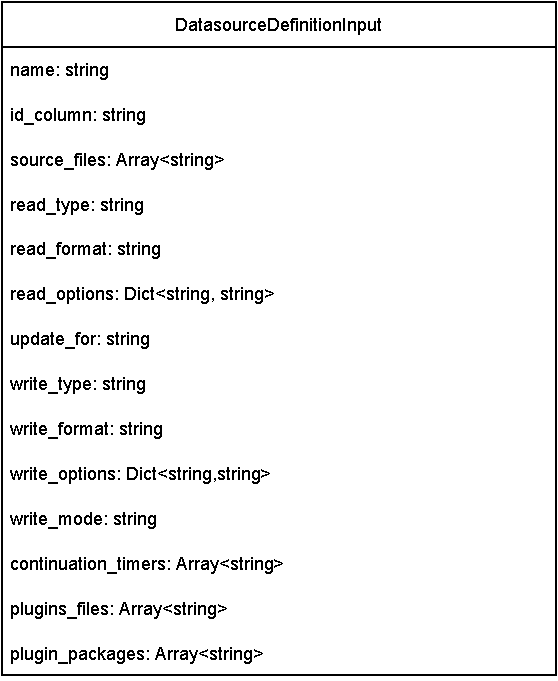
\includegraphics[width=.65\textwidth]{Grafiken/Umsetzung-Definition-Input.pdf}
    \caption{Felder Datenquellen-Eingabe}
    \label{fig:datasource-definition-input}
\end{figure}

\subsection{Hochladen von Dateien}

Für jede Datenquelle können Quell- oder Plugin-Dateien hochgeladen werden.
Um eine hochgeladene Datei in der Datenquelle auch zu verwenden, muss der Schlüssel, unter dem die Datei hochgeladen wird, in der entsprechenden Liste entweder unter "`source\_files"' oder unter "`plugin\_files"' hinzugefügt werden.
Alternativ können auch die Namen unter denen bereits Dateien für die Datenquelle gespeichert wurden in die Listen eingefügt werden.

Bei der Verarbeitung der Eingabe prüft der API-Service für jeden Eintrag der Listen, ob eine Datei mit diesem Schlüssel hochgeladen wurde.
Ist das der Fall, wird die entsprechende Datei in das HDFS hochgeladen.
Der Name, unter dem die Datei gespeichert wird, setzt sich aus der Nummer der Revision, dem vergebenen Schlüssel und der Endung der Datei zusammen.
Lädt man also eine bei der ersten Erstellung einer DatasourceDefinition eine Datei "`data.json"' mit den Schlüssel "`file"' hoch, wird diese als "`r000\_file.json"' im "`sources"'-Ordner der DarasourceDefinition gespeichert.
Analog werden Plugin-Dateien genauso behandelt.

Wenn keine Datei in der Anfrage gefunden wurde, wird geschaut, ob im HDFS eine Datei mit dem Namen existiert.
Wird eine Datei gefunden, wird der Name an die neue Revision angehangen.
Es ist wichtig zu beachten, dass alle Dateien der alten Revision, die nicht explizit in einer der Listen angegeben werden, nicht in der neuen Revision verwendet werden.
Sie bleiben jedoch gespeichert und können später wieder hinzugefügt werden.
Da die Dateien nach den Datenquellen aufgeteilt sind, ist es aktuell nicht möglich Plugins oder Quell-Dateien in anderen Datenquellen wieder zu verwenden.
Hier müsste man die Datei für jede Datenquelle hochladen.

\section{Continuation-Service}

Der Continuation-Service führt durchgehend eine Schleife zum Überprüfen der Datenquellen aus.
Bei der Prüfung wird immer der Status des aktuellsten IngestionEvent betrachtet.
Je nach Datenquelle wird dann entschieden, ob eine Ingestion gestartet werden soll.
Die Logik der Schleife besteht aus drei Teilen, wovon zwei die Datenquellen prüfen und einer die Zeit steuert, nachdem die Schleife erneut ausgeführt wird (\cref{algo:ci-loop}).
Das soll nur maximal jede Minute geschehen, da auch keine schnellere Ausführung über die Timer definiert werden kann.

Im ersten Teil werden alle Datenquellen einer Datenstrom-Ingestion kontrolliert.
Für diese wird eine neue Ingestion gestartet, wenn der Status "`FINISHED"' ist.
Der Status "`STOPPED"' bedeutet, dass die Ausführung mit Absicht beendet wurde und manuell gestartet werden muss.

Der zweite Teil überprüft alle Datenquellen, bei denen ein oder mehrere Timer gesetzt wurden.
Wenn der Status des letzten IngestionEvents nicht "`STOPPED"' oder "`FINISHED"' ist, wird die Überprüfung dieser Quelle abgebrochen.
Ansonsten wird jeder Timer mit dem aktuellen Zeitpunkt verglichen.
Hier wird die Methode $is_now$ verwendet.
Sie wird durch eine Python-Bibliothek bereitgestellt und prüft ob ein Cron-Timer, die auch für die kontinuierliche Ingestion eingesetzt werden, zum aktuellen Zeitpunkt zutrifft.
Trifft der Timer zu, wird eine Ingestion für die Datenquelle gestartet und sofort die nächste Datenquelle überprüft.

Der dritte Teil kontrolliert die Ausführungshäufigkeit.
Dazu wird am Anfang der Schleife der Startzeitpunkt gespeichert.
Nachdem alle Überprüfungen beendet wurden, wird auch der Endzeitpunkt gespeichert.
Wenn die Differenz der beiden geringer ist als eine Minute, wird die Schleife für die Dauer der Differenz angehalten.
Damit ist sichergestellt, das sie nicht häufiger als einmal pro Minute ausgeführt wird.

\begin{algorithm}
    \caption{Continuation loop}
    \label{algo:ci-loop}
    
    \KwData{-}
    \KwResult{-}
    
    $loopStart \gets$ current\_time() \;
    
    $streams \gets$ all\_datasource\_definition\_of\_type\_stream() \;
    \ForAll {$definition$ in $streams$} {
        $event \gets definition.last\_ingestion$ \;
        \If {$event.state$ is FINISHED} {
            publish\_run\_event\_for($definition.id$) \;
        }
    }
    
    $timed \gets$ all\_datasource\_definitions\_with\_timers() \;
    \ForAll {$definition$ in $timed$} {
        $event \gets definition.last\_ingestion$ \;
        $timers \gets definition.revision.continuation\_timers$  \;
        \If {$event.state$ is STOPPED or FINISHED} {
            \ForAll {$timer$ in $timers$} {
                \If {is\_now($timer$)} {
                    publish\_run\_event\_for($definition.id$) \;
                    \textbf{break}
                }
            }
        }
    }

    $loopEnd \gets$ current\_time() \;
    $loopDuration \gets loopEnd - loopStart$ \;
    \If {$loopDuration < 60$} {
        sleep($60 - loopDuration$) \;
    }

\end{algorithm}


\section{Ingestion-Service}

Wie in \fref{sec:entw-ingestion} beschrieben, wird für ein Event ein Prozess gestartet.
Der Name der Topic des Events zum Starten einer Ingestion ist "`dls\_\_ingestion\_\_run"'.
In \fref{sec:ingestion-run} wird der detailliere Ablauf mit den verschiedenen Wegen für Read- und SaveTypes beschrieben.
Vorher werden die benötigt Grundlagen zur Ausführung erläutert.

\subsection{Berechnen und Speichern der Änderungsdaten}
Um Änderungen in eine Delta Tabelle zu übernehmen, müssen die Änderungsdaten in einem Format sein, dass Aufschluss darüber gibt, welche Daten hinzugefügt, welche geändert und welche gelöscht worden sind.
Das hier verwendete Format muss genau dem gleichen Schema entsprechen, wie die original Daten.
Zusätzlich soll eine Spalte oder ein Feld auf der obersten Eben mit dem Namen "`cd\_deleted"' vorhanden sein.
Es enthält einen Boolean-Wert, der sagt, ob der Eintrag aus den Daten gelöscht wurde oder nicht.
Der Datensatz mit den Änderungsdaten darf außerdem nur geänderte Daten enthalten.
Aus diesem Format können, wie später gezeigt, die drei Operationen abgeleitet werden.

Um nicht auf ein externes Change-Data-Capture-System angewiesen zu sein, gibt es eine interne Lösung, die auf alle (semi-)strukturierten Daten angewendet werden kann.
Der \cref{algo:delta-calc} zeigt, wie aus zwei DataFrames die Änderungsdaten erzeugt werden.
Als Eingabe werden ein linkes DataFrame, mit dem aktuellen internen Stand, eine rechtes DataFrame, mit den neuen Daten und der Name der Id-Spalte benötigt.
Das Ergebnis ist ein DataFrame mit allen aktualisierten Datensätzen.
Es hat das gleiche Schema wie die Ursprungsdaten, aber mit der zusätzlichen Spalte, die Auskunft darüber gibt, ob ein Datensatz gelöscht wurde.

\begin{algorithm}
    \caption{Deltaberechnung}
    \label{algo:delta-calc}
    \KwData{leftDataFrame, rightDataFrame, idColumn}
    \KwResult{changeDataFrame}
    $leftDataFrame \gets$ add column with row hash \;
    $leftDataFrame \gets$ prefix column names with "`left\_"' \;
    $rightDataFrame \gets$ add column with row hash \;
    $rightDataFrame \gets$ prefix columnnames with "`right\_"' \;

    $changeDataFrame \gets$ full join over $idColumn$ of $leftDataFrame$ and $rightDataFrame$ \;

    $changeDataFrame \gets$ remove all rows where $left\_hash$ equals $right\_hash$ \;

    $changeDataFrame \gets$ remove hash columns

    $changeDataFrame \gets$ add row $cd\_deleted$ \;
    \eIf{$right\_idColumn$ is $null$}{$cd\_deleted = true$}{$cd\_deleted = false$}

    $changeDataFrame \gets$ merge left and right $idColumn$ into one $idColumn$
    \eIf{$left\_idColumn$ is not $null$}{$idColumn = left\_idColumn$}{$idColun = right\_idColumn$}

    $changeDataFrame \gets$ merge remaining columns with left and right value by always taking the right and removing prefix

\end{algorithm}

Das Einpflegen der Änderungen wird über die Delta Lake API gelöst.
Dazu werden die Änderungsdaten mit den aktuellen Daten über die Id-Spalte zusammengeführt.
Dabei können verschieden Fälle definiert werden.
Wenn die Ids einer Zeile gleich sind und die Spalte "`cd\_deleted"' $true$ enthält, wird die Zeile aus den Daten gelöscht, ansonsten wird der Datensatz aktualisiert.
Wenn die Ids nicht übereinstimmen und die Spalte "`cd\_deleted'" $false$ ist, dir der Datensatz als neue Zeile eingefügt.

\subsection{Plugins verwalten}
Für jede Ingestion wird auf dem Speichersystem des Mircoservices ein temporärer Ordner angelegt, in den die Plugins und deren Abhängigkeiten installiert werden.
Nach der Installation wird noch eine Datei angelegt, die für alle Pakete die Versionen enthält.
Das dient dazu, bei einer erneuten Ausführung auf dem Service nicht alle Pakete neu installieren zu müssen, sondern nur die mit geänderten Version.
Das beschleunigt die Ausführung der Ingestion.
Zum Schluss wird der Ordner, in den die Pakete installiert wurden an den Python-Pfad mit angehangen.
Damit wird dieser während der Ausführung manipuliert und die Pakete sind verfügbar.
Da jede Ingestion in einem eigenen Prozess beeinflussen die Änderungen an dem Python-Pfad den Ingestion-Service oder andere Prozesse nicht.

Im zweiten Schritt wird jede Python-Datei im Pluginordner als Modul geladen.
Die im Modul verfügbaren Methoden werden dann überprüft, ob sie auf eine Definition der möglichen Plugins passen.
Dazu wird der \fref{algo:check-method} verwendet.
Diesem werden das geladene Modul, ein Name der Methode, ein optionaler Rückgabetyp der Methode und eine Liste von Parameter, bei denen Name und Typ definiert ist.
Zur Überprüfung können alle Methoden in dem Modul auf ihren Namen geprüft werden.
Wenn eine Methode gefunden wurde, wird eine Signatur erzeugt und mit der übergebenen Definition verglichen.
Das Ergebnis sagt dann, ob diese Methode ein Plugin ist oder nicht.

Jedes geladene Modul wird auf Load- oder AfterLoad-Methoden geprüft.
Eine gefundene Load-Methode überschreibt immer die letzte gefunden, da bei einer Ausführung auch das Ergebnis dieser Methoden überschrieben werden würde.
Die AfterLoad-Methoden dagegen werden in einer Liste gespeichert.


\begin{algorithm}
    \caption{Pluginmethode überprüfen}
    \label{algo:check-method}

    \KwData{$plugin$, $name$, $return\_type$, $parameters$}

    \KwResult{$matches$}

    \If{plugin has NOT method with name $name$}{
        \Return{false}
    }

    $signature \gets$ signature of mehtod $name$

    \If{$return\_type$ is given AND $signature$ NOT returns type of $return\_type$}{
        \Return{false}
    }

    \ForAll{$param$ in $parameters$}{
        \If{$signature$ has NOT a parameter named $param.name$}{
            \Return{false}
        }

        \If{$signature$ type of parameter $param.name$ is NOT $parameter.type$}{
            \Return{false}
        }
    }

    \Return{true}

\end{algorithm}

\subsection{Ausführung der Ingestion}
\label{sec:ingestion-run}
Die Ausführung startet mit der Initialisierung, die die für die Ingestion benötigte Daten lädt.
Das ist zum Beispiel die DatasourceDefinition zu der Id aus den Events.
Danach wird entschieden ob eine Ingestion über Spark notwendig ist.
Hier spielt der Lesetyp eine große Rolle.
Eine Ingestion von Datendateien benötigt keine Spark, es werden einfach direkt die Dateien in das entsprechende Zielverzeichnis kopiert.
Für alle anderen Typen wird im nächsten Schritt die Ingestion vorbereitet.
Es werden die Plugins aus dem HDFS geladen und eine SparkSession erstellt.
Das Laden der Daten in ein DataFrame geschieht anschließend entweder über ein Plugin in oder das Standardvorgehen.
Falls auch After-Load-Plugins vorhanden sind werden diese ausgeführt.
Für die geladenen Daten wird dann entschieden, ob es sich um Änderungsdaten handelt oder welche berechnet werden müssen.
Je nach Schreib-Typ werden dann die Daten beziehungsweise Ändeurngsdaten gespeichert.
Für Datenströme wird am Ende noch ein Hintergrund Task gestartet, der auf Kafka Events zum stoppen dieser Ingestion wartet.
Hierfür wird die Topic "`dls\_\_ingestion\_\_stop\_ingestion"' mit der Id als Wert verwendet.
Wenn die Ingestion beendet wurde, wird zum Schluss die SparkSession gestoppt.

\begin{figure}
    \centering
    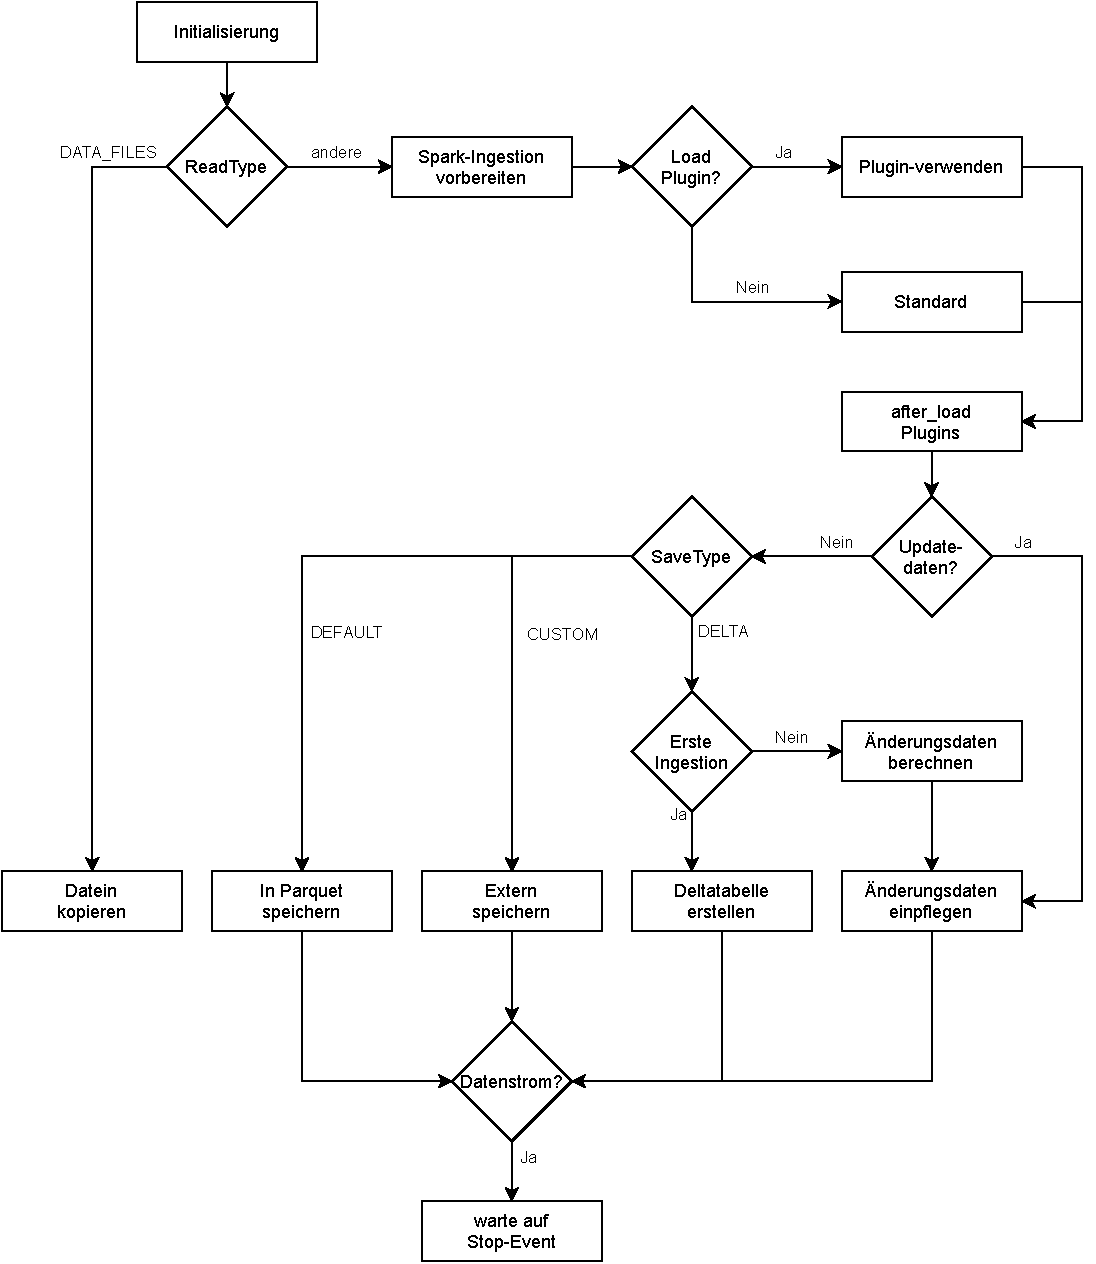
\includegraphics[width=\textwidth]{Grafiken/Umsetzung-Ingestion-Ablauf.pdf}
    \caption{Ablauf einer Ingestion}
    \label{fig:umsetz-ingestion-ablauf}
\end{figure}
\chapter{Evaluierung}

Die Evaluierung der Ingestion-Schnittstelle besteht aus zwei Teilen.
Im ersten Schritt wird geprüft, ob alle Anforderungen aus \cref{sec:anf} erfüllt wurden.
Dabei wird unterschieden in Anforderungen, deren Erfüllung durch die Betrachtung der Umsetzung bereits festgestellt werden kann und solche, bei denen ein funktionaler Test notwendig ist.
Im zweiten Teil werden in einem Benchmark verschiedene Parameter gemessen, um einen Überblick zu geben, wie sich das System bei Verwendung verhält.

\section{Erfüllung der Anforderungen}

Die ersten Anforderung die geprüft werden können, sind ANF\_12, ANF\_13 und ANF\_14, welche die Architektur beziehungsweise das Design des Systems betreffen.
Die Ingestion bietet eine REST-Schnittstelle, wie durch die Anforderung gefordert.
Die drei Microservices sind nicht voneinander abhängig und die Kommunikation mit Kafka ist so flexibel, dass es kein Problem gibt neue Services zu integrieren.

Auch ANF\_09, das Speichern von Änderungen, ist durch die Verwendung von Delta Lake gegeben.
Die Erfüllung der restlichen Anforderungen muss durch Tests überprüft werden.
Hierzu werden Tests verwendet, die das komplette System im Zusammenhang überprüfen.
Hier bedeutet das, dass mehrere Ingestions ausgeführt werden, die alle Funktionen abdecken.
Mit den folgenden Schritten kann die korrekte Funktion einer Ingestion getestet werden: \begin{enumerate}
    \item Erstellen einer Datenquelle, zum Beispiel JSON-Dateien oder Postgres-Ta\-bellen, die in der Ingestion verwendet wird.
    \item Erstellen einer DatasourceDefinition für die Datenquelle.
    \item Vergleichen der DatasourceDefinition aus der Datenbank des Systems mit einer vordefinierten Soll-Definition.
    \item Starten der Ingestion.
    \item Vergleichen der Daten im System nach der Ingestion mit einem vordefinierten Soll-Datensatz
\end{enumerate}
Mit diesem Vorgehen kann auch die Aktualisierung von Daten getestet werden.
Dazu muss es zweimal hintereinander ausgeführt werden.
Im ersten Durchlauf werden die initialen Daten geladen und im zweiten wird dann entweder die gleiche Datenquelle mit veränderten Daten oder Änderungsdaten aus einer Updatequelle geladen.

\subsection{Durchgeführte Tests}
\label{sec:tests-actual}
Nachfolgend werden die durchgeführten Tests geschildert.
Die ersten Tests sollen zeigen, dass sowohl das Laden von veränderten Daten als auch von Änderungsdaten für strukturierte und unstrukturierte Daten funktioniert.
Damit wird auch indirekt die korrekte Ingestion überprüft.

Ein verwendeter Datensatz muss aus einer Mindestanzahl an Einträgen bestehen, die alle möglichen Operation bei einer Änderung abdecken.
Der erste Eintrag bleibt in den Update-Daten unverändert, der zweite wird gelöscht und der dritte wird in einem Feld verändert.
Zusätzlich muss noch ein weiterer Eintrag hinzugefügt werden.
Damit Änderungen berechnet und eingepflegt werden können muss ein Feld festgelegt werden, dass als Id verwendet wird.
Hier muss auch der Fall geprüft werden, dass die Id sich in einem verschachtelten Feld befindet.

Für den Test von strukturierten Daten wird eine Postgres Datenbank und für semistrukturierte JSON-Dateien verwendet.
Damit werden der Upload von Dateien und das Laden von Daten aus einer Datenquelle abgedeckt.
Für beide wird sowohl die Ingestion von veränderten Daten der gleichen Quelle als auch Änderungsdaten ausgeführt.
Dabei werden jeweils eine Delta-Tabelle und Parquet als Speicherziel verwendet.
Das Speichern in einem externen Ziel wird hier nicht getestet, da die Versionierung nur für interne Speicher unterstützt wird.
Der erfolgreiche Abschluss der Tests hat gezeigt, dass diese Ingestion-Abläufe bei veränderten Daten funktionieren: \begin{itemize}
    \item neuen Stand einer Datenquelle in Parquet speichern,
    \item Änderungsdaten aus einer externen Quelle in Bestandsdaten aus Parquet einpflegen,
    \item Änderungsdaten aus einem neuem Stand einer Datenquelle berechnen und in einer Delta-Tabelle speichern und
    \item Ändeurngsdaten aus einer externen Quelle in eine Delta-Tabelle einpflegen.
\end{itemize}

Bei den Tests für weitere Quellen genügt es nur noch eine Ingestion auszuführen.
Hier werden die Ingestion aus einem Kafka-Datenstrom und aus einer REST-Api überprüft.
Die Ingestion des Datenstroms verwendet dabei ein After-Load-Plugin, um die tatsächlichen Daten aus der Nachricht zu extrahieren.
Das Load-Plugin wird bei der Ingestion aus einer REST-API mit geprüft.
Auch diese Tests sind erfolgreich durchgelaufen.
\section{Benchmarks}

Benchmarks sind ein allgemeines Mittel um Systeme zu bewerten.
Dabei werden festgelegte Operationen ausgeführt und bestimmte Parameter, die einen Interessieren gemessen.
Im Big-Data-Bereich wird meistens die Menge der Daten, die verarbeitet werden könne bewertet.
Hier sind Beispiele der Bigdatabench \parencite{bigdatabench} oder der TPCx-BB\footnote{http://tpc.org/tpcx-bb/default5.asp} und TCPx-HS\footnote{http://tpc.org/tpch/default5.asp}.
Diese Messen verschiedene Verarbeitungsoperationen mit großen Datenmengen auf einem bestehenden System.
Teilweise werden zusammen mit der Datenmenge auch Kosten oder Stromverbrauch gemessen.
Neben diesen Benchmarks kann auch die Qualität des Ergebnisses einer bestimmten Verarbeitungspipline gemessen werden.

Für die Bewertung der Ingestion-Schnittstelle sind solche Benchmarks nicht geeignet.
Da die Geschwindigkeit oder Menge der Datenverarbeitung von Cluster zu Cluster unterschiedlich, die Schnittstelle aber für verschiedene Cluster eingesetzt werden soll.
Hier bieten sich relative Vergleiche als eine bessere Lösung an.
Dazu werden verschieden große Datensätze unter den gleichen Bedingungen in das System geladen und die Dauer der Ingestion und der verbrauchte Festplattenplatz gemessen.

\subsection{Benchmark-Vorgehen}
Ein wichtiger und ausschlaggebender Punkt der Ingestion ist die Versionierung und Verarbeitung von Änderungsdaten.
Daraus folgt, dass hier für die Benchmarks das Verhalten beim Laden von Updates interessant ist.
Dafür werden die vier Ingestion-Abläufe aus \cref{sec:tests-actual}, Updates in Parquet, Änderungsdaten in Parquet, Updates in eine Delta-Tabelle und Änderungsdaten in eine Delta-Tabelle mit schrittweise erhöhten Datenmengen durchlaufen.
Zusätzlich werden sowohl strukturierte als auch semistrukturierte Daten verwendet.

Die Beispieldatensätze wurden selber generiert um die genaue Anzahl und Inhalt bestimmen zu können.
So bleiben die Daten auch zwischen den Strukturen vergleichbar.
Zur Generierung wurde das Tool Synth\footnote{https://www.getsynth.com/} verwendet.
Bei diesem wird in einer JSON-Datei ein Schema definiert.
In dem Schema kann für ein Feld aus verschiedenen Generatoren gewählt werden, die zufällige oder feste Werte in den Daten erzeugen.
Es ist auch in der Lage realitätsnahe Daten wie Namen oder E-Mail-Adressen zu generieren.
Als Speicherziel können entweder JSON-Dateien oder einige Datenbanken gewählt werden.

Bei der Datengenerierung wird zuerst ein initialer Datensatz erstellt.
Für diesen werden dann eine bestimmte Anzahl an Änderungen, Löschungen und Einfügungen erzeugt, die einmal in einer Kopie des Datensatzes als neuer Datensatz angewendet werden und einmal in einem Datensatz in Form von Änderungsdaten gespeichert werden.
Die Menge der Daten wird durch vier Parameter gesteuert.
Der erste ist die Anzahl an Zeilen im initialen Datensatz.
Die anderen drei legen die Änderungen, Löschungen und Einfügungen fest.
Sie werden in Prozent angegeben und werden auf Basis der Anzahl an Zeilen berechnet.

Für die Durchführung eines Benchmarks werden dann die folgenden Schritte ausgeführt.
Dabei sind fast alle Schritte gleich.
Nur Schritt vier und fünf unterscheiden sich bei der Verwendung einer veränderten Tabelle oder von Änderungsdaten.
Für die Benchmark-Messungen kann die Dauer aus den Ingestion-Events berechnet werden, da diese die Start- und Endzeit enthalten.
Die Größe der Dateien wird kann über eine WebHDFS-Abfrage der Eigenschaften des entsprechenden Ordners geschehen, da sowohl Parquet als auch die Delta-Tabelle in HDFS gespeichert werden.
\begin{enumerate}
    \item Erstellen einer DatasourceDefinition für die initialen Daten.
    Bei Postgres wird die Tabelle angegeben und bei JSON werden die entsprechenden Dateien hochgeladen. 
    \item Führe die erste Ingestion mit der Datenquelle aus.
    \item Überprüfe, ob die Anzahl der Einträge in den geladenen Daten korrekt ist und erfasse Benchmark-Parameter für die initialen Daten.
    \item Erstelle DatasourceDefinition für Änderungsdaten oder ändere die bestehende DatasourceDefinition, die veränderten Daten zu benutzen.
    Damit bei mehrfachen Benchmarks nicht immer wieder neu die Änderungen gemacht werden müssen, wird das dadurch simuliert, dass die Datenquelle der DatasourceDefinition angepasst wird. Für Postgres wird hier einfach die Tabelle geändert und für JSON werden die Dateien mit den neuen Daten hochgeladen und die alten nicht in die Liste der Quelldateien übernommen.
    \item Führ entweder eine erneute Ingestion der Datenquelle aus oder führe die erste Ingestion für die Änderungsdaten aus.
    \item Überprüfe, ob die Anzahl der Daten korrekt ist und erfasse Benchmark-Parameter für die veränderten Daten.
\end{enumerate}

Die durchgeführten Benchmarks sollen zwei verschiedene Fälle abbilden.
Der erste Fall ist eine Datenquelle in der häufig Änderungen vorkommen.
Hier werden 80\% Änderungen, 20\% Löschungen und 40\% Löschungen verwendet.
Im zweiten Fall geht es darum, dass hauptsächlich neue Daten eingefügt werden und Änderungen und Löschungen werden selten gemacht.
Dafür werden 5\% Änderungen, 5\% Löschungen und 80\% Einfügungen angewendet.
Die Benchmarks für ein Speicherziel, also Parquet oder Delta-Tabelle, werden immer zusammen ausgeführt.
Das heißt, dass die Ingestion von aktualisierten Daten und von Änderungsdaten direkt hintereinander geschieht.
Dadurch kann eine weiter Überprüfung mit eingebaut werden.
Da das Speicherziel gleich ist muss für beide Durchläufe auch die Speichergröße der initialen Daten gleich sein.

Als Ziele der Datengenerierung und somit auch als Datenquellen werden wie bei den Tests Postgres und JSON-Dateien verwendet.
Die Daten selber bestehen aus jeweils 10 Feldern, wovon eines ein fortlaufenden Nummer als Id ist, eines ein Datum enthält und die anderen mit einem Zufälligen 32-Zeichen langen Text befüllt werden.
Bei den semistrukturierten Daten werden außerdem die Felder ineinander verschachtelt.
Die Anzahl an Einträgen wird von 1000 bis 7.500.000 gesteigert.
Dabei wird mit 1000, der nächste Schritt ist dann 2500, dann folgen 5000 Einträge und danach 7500.
Das wird dann für alle weiteren 10er-Potenzen wiederholt.

\subsection{Benchmark-Ergebnisse}

Die Benchmarks konnten nur auf einem lokalen Spark-Cluster mit einem Worker ausgeführt werden.
Diesem standen 8 Kerne und 20 Gigabyte Arbeitsspeicher zur Verfügung.
Es wurde auch probiert diesen Worker in zwei, mit jeweils der Hälfte der Ressourcen, auf zu teilen.
Bei dieser Konfiguration konnten die Benchmarks aber nicht für Zeilenanzahl ab 1.000.000 erfolgreich beendet werden, da die Ressourcen nicht ausreichend waren.
Aufgrund des verwendeten Spark-Clusters hat die Betrachtung der absoluten Zahlen keine große Aussagekraft.
Diese ändern sich mit dem Spark-Cluster und sind nur sinnvoll, wenn der Benchmark auf dem System ausgeführt wird, dass auch beim Betrieb zum Einsatz kommen soll.
Eine der Kern-Funktionen ist die Versionierung.
Daher werden die Benchmark-Ergebnisse mit dem Ziel verglichen, Aussagen über diese Funktion zu treffen.
Dazu wird jeweils ein Faktor für die zwei Fälle und die Quelle wie folgt berechnet:
\begin{align*}
    & p_t: \text{Zeit beim Speichern in Parquet, ohne Versionierung} \\
    & d_t: \text{Zeit beim Speichern in Delta-Tabelle, mit Versionierung} \\
    & f_t = d_t / p_t \\ \\
    & p_s: \text{Speicherverbrauch in Parquet, ohne Versionierung} \\
    & d_s: \text{Speicherverbrauch in Delta-Tabelle, mit Versionierung} \\
    & f_s = d_s / p_s \\ \\
\end{align*}
Diese Werte werden für die zweite Ingestion für beide Fälle mit jeweils aktualisierten Daten oder Änderungsdaten berechnet.
Da die initialen Daten in beiden Fällen gleich sind, werden die Faktoren hierfür nur einmal berechnet.

Der Wert der Faktoren kann folgendermaßen interpretiert werden: \begin{align*} 
    & f_t > 1: \text{Die Ingestion mit Versionierung ist langsamer als ohne} \\
    & f_t = 1: \text{Beide Ingestions sind gleich schnell} \\
    & f_t < 1: \text{Die Ingestion mit Versionierung ist schneller als ohne} \\ \\
    & f_s > 1: \text{Die Ingestion mit Versionierung verbraucht mehr Speicherplatz} \\
    & f_s = 1: \text{Beide Ingestions verbrauchen gleich viel Speicher} \\
    & f_s < 1: \text{Die Ingestion mit Versionierung verbraucht weniger Speicherplatz}
\end{align*}

In den gezeigten Diagrammen werden nur die Ergebnisse ab 100.000 Zeilen gezeigt, da die Unterschiede vorher zu klein sind, um sie erkennbar dar zu stellen.
Alle Ergebnisse können in den Tabellen in \cref{sec:benchmark-tables} nachgelesen werden.


\subsubsection{Dauer der Ingestion}
Beschreibung
\begin{figure}
    \centering
    \label{fig:eval-time-c}
    \subfigure[Dauer aus PostgreSQL]{
        \includesvg[inkscapelatex=false,width=0.6\textwidth]{Grafiken/Evaluierung/Evaluierung_Zeit_Sql-Initial}
        \label{fig:eval-time-sql-i}
    }
    \subfigure[Dauer aus JSON-Dateien]{
        \includesvg[inkscapelatex=false,width=0.6\textwidth]{Grafiken/Evaluierung/Evaluierung_Zeit_Json-Initial}
        \label{fig:eval-time-json-i}
    }
    \caption{Erste Ingestion}
\end{figure}

\begin{figure}
    \centering
    \label{fig:eval-time-c}
    \subfigure[Dauer aus PostgreSQL]{
        \includesvg[inkscapelatex=false,width=0.8\textwidth]{Grafiken/Evaluierung/Evaluierung_Zeit_Sql-Updated}
        \label{fig:eval-time-sql-u}
    }
    \subfigure[Dauer aus JSON-Dateien]{
        \includesvg[inkscapelatex=false,width=0.8\textwidth]{Grafiken/Evaluierung/Evaluierung_Zeit_Json-Updated}
        \label{fig:eval-time-json-u}
    }
    \caption{Ingestion aus aktualisierten Daten}
\end{figure}

\begin{figure}
    \centering
    \label{fig:eval-time-c}
    \subfigure[Dauer aus PostgreSQL]{
        \includesvg[inkscapelatex=false,width=0.8\textwidth]{Grafiken/Evaluierung/Evaluierung_Zeit_Sql-Cdc}
        \label{fig:eval-time-sql-c}
    }
    \subfigure[Dauer aus JSON-Dateien]{
        \includesvg[inkscapelatex=false,width=0.8\textwidth]{Grafiken/Evaluierung/Evaluierung_Zeit_Json-Cdc}
        \label{fig:eval-time-json-c}
    }
    \caption{Ingestion aus Updatequelle}
\end{figure}

\chapter{Zusammenfassung und Ausblick}

Die Aufgabenstellung dieser Arbeit war die Entwicklung einer Ingestion-Schnitt\-stelle für ein Data-Lake-System, dass im Kontext des HIT-Instituts an der Hochschule Niederrhein angewendet werden soll.
An diesem Institut werden Daten aus verschiedenen Quellen erfasst.
Es gibt klassische Datenbank-Systeme, Dateien oder REST-APIs.
Der Data Lake soll die zentrale Speicherlösung sein und Verarbeitungsprozesse unterstützen.
Dazu ist es neben der Unterstützung verschiedener Datenquellen auch nötig die Daten zu versioniern.
Dadurch verringert sich der Aufwand bei der weiteren Verarbeitung, da nur Änderungen betrachtet werden müssen.

In der vorliegenden Arbeit wurde eine generische Ingestion-Schnittstelle mit Versionierung für Data-Lake-Systeme entwickelt und mit funktionalen Tests und Benchmarks evaluiert.
Dafür wurde neben der Entwicklung der bestehende Prototyp des Data Lake auf eine Microservice-Archi\-tektur umgebaut.
Es wurden außerdem existierende Data-Lake-Systeme betrachtet und bewertet, ob diese als Lösung für die Problemstellung dienen könnten.
Daraus ergab sich, dass eine Eigenentwicklung notwendig ist.

Die Ingestion-Schnittstelle besteht aus drei Microservices.
Der Ingestion-Ser\-vice verwaltet das Laden von Daten in das System.
Dabei erlaubt die Verwendung von Spark und einem Plugin-System das Laden von Daten aus jeder Quelle.
Die kontinuierliche Ausführung von Ingestions wird durch den Continuation-Service sichergestellt.
Benutzer können über den API-Service mit der Ingestion-Schnittstelle interagieren.
Dieser besteht aus der Integration der neuen API in den Server des Prototyps.
Dadurch bleibt das System mit der Verwendung der alten API kompatibel.
Aus der Eingabe, die ein Benutzer an die API sendet, wird ein generelles Metadatenmodell aufgebaut.

Das Metadatenmodell zur Definition einer Datenquelle enthält alle Informationen über die Datenquelle, verwendete Plugins und zugehörige Ingestions.
Über dieses Modell werden die Informationen zu den Ingestions zwischen den Microservices ausgetauscht.

Neben der Ingestion-Schnittstelle besteht der Data Lake aus weiteren Komponenten.
Ein Kafka-Cluster wird für die Kommunikation im Data-Lake-System eingesetzt.
Diese kann auch für die Anbindung von Datenströmen verwendet werden.
Die Daten, die in den Data Lake geladen wurden, werden in einem HDFS gespeichert.
Daten mit Versionierung werden in einer Delta-Tabelle des Delta Lake abgelegt.
Für unversionierte Daten wird entweder das Parquet- oder, bei unstrukturierten Daten, das Ursprungsformat der Daten benutzt.
Für die Verwaltung von Metadaten kommt eine MongoDB-Datenbank zum Einsatz.
Die Datenverarbeitung geschieht über ein Spark-Cluster.

Die Evaluierung der Ingestion-Schnittstelle wurde in einem durch die gegebene Hardware möglichen Rahmen durchgeführt.
Hierfür stand kein leistungsstarkes Cluster zur Verfügung, um absolute Aussagen über die Leistung der Ingestion-Schnittstelle treffen zu können.
Daher ist lediglich ein relativer Vergleich ausgeführt worden, der Aussagen zur Skalierbarkeit des Ansatzes erlaubt.
Dabei wurden Benchmarks für verschiedene Datenmengen mit strukturierten und semistrukturierten Daten in zwei Szenarien ausgeführt.
Die Szenarien bilden dabei eine Situation, in der viele Änderungen an Daten geschehen und eine Situation, in der hauptsächlich Daten hinzugefügt werden ab.

Durch die Benchmarks und Tests wurde gezeigt, dass mit dieser Arbeit die Entwicklung der Ingestion-Schnittstelle noch nicht vollständig abgeschlossen ist.
Die implementierte Berechnung von Änderungsdaten ist in bestimmten Fällen sehr langsam.
Auch die Darstellung von Änderungen in verschachtelten Daten könnte durch ein anderes Vorgehen optimiert werden.
Somit ist die Versionierung in der Ingestion-Schnittstelle ein Thema, dass in einer anschließenden Arbeit genauer betrachtet werden kann.

Weiterhin sind die Metadaten, die während der Ingestion gesammelt werden, nicht ausreichend.
Um eine aussagekräftige Suche, Exploration und Analyse der Daten durchführen zu können, müssen direkt nach dem Laden weitere Metadaten automatisch extrahiert oder manuell durch einen Benutzer hinzugefügt werden.
Diese könnten zum Beispiel Informationen über den Inhalt oder die Struktur der Daten beinhalten.
Die in dieser Arbeit entwickelte Ingestion-Schnittstelle ist modular und erweiterbar aufgebaut, so dass in zukünftigen Arbeiten entsprechende Erweiterungen umgesetzt werden können.
\printbibliography

\appendix
\label{sec:benchmark-tables}
Nachfolgend sind alle Ergebnisse der Benchmarks aufgelistet.
Zeiten sind dabei immer im Format Minuten:Sekunden.
In den Spaltenüberschriften werden die drei Buchstaben mit folgenden Bedeutungen verwendet:
\begin{description}
    \item[I]: Initiale Ingestion
    \item[U]: Ingestion mit aktualisierten Daten
    \item[C]: Ingestion mit Änderungsdaten
\end{description}

\begin{table}
    \centering
    \begin{tabular}{|r|r|r|r|r|r|r|}
        \hline
        \textbf{Zeilen} & \textbf{Speicher I} & \textbf{Zeit I} & \textbf{Speicher U} & \textbf{Zeit U} & \textbf{Speicher C} & \textbf{Zeit C} \\ \hline
        1,0e+3 & 0,96 MB       & 00:07 & 0,83 MB       & 00:07 & 0,84 MB       & 00:10 \\ \hline
        2,5e+3 & 2,39 MB       & 00:07 & 2,11 MB       & 00:07 & 2,11 MB       & 00:10 \\ \hline
        5,0e+3 & 4,75 MB       & 00:07 & 4,22 MB       & 00:07 & 4,22 MB       & 00:10 \\ \hline
        7,5e+3 & 7,12 MB       & 00:08 & 6,29 MB       & 00:08 & 6,30 MB       & 00:10 \\ \hline
        1,0e+4 & 9,48 MB       & 00:08 & 8,47 MB       & 00:08 & 8,47 MB       & 00:10 \\ \hline
        2,5e+4 & 23,66 MB      & 00:08 & 21,14 MB      & 00:08 & 24,45 MB      & 00:10 \\ \hline
        5,0e+4 & 47,30 MB      & 00:09 & 52,77 MB      & 00:08 & 52,30 MB      & 00:11 \\ \hline
        7,5e+4 & 70,94 MB      & 00:09 & 79,15 MB      & 00:09 & 79,23 MB      & 00:12 \\ \hline
        1,0e+5 & 94,57 MB      & 00:09 & 105,38 MB     & 00:09 & 105,70 MB     & 00:13 \\ \hline
        2,5e+5 & 236,39 MB     & 00:11 & 264,49 MB     & 00:12 & 264,71 MB     & 00:16 \\ \hline
        5,0e+5 & 474,70 MB     & 00:15 & 531,68 MB     & 00:16 & 529,78 MB     & 00:20 \\ \hline
        7,5e+5 & 711,06 MB     & 00:18 & 796,23 MB     & 00:20 & 795,45 MB     & 00:25 \\ \hline
        1,0e+6 & 949,38 MB     & 00:21 & 1.060,58 MB   & 00:23 & 1.060,46 MB   & 00:29 \\ \hline
        2,5e+6 & 2.373,41 MB   & 00:40 & 2.651,87 MB   & 00:48 & 2.657,99 MB   & 01:08 \\ \hline
        5,0e+6 & 4.748,75 MB   & 01:16 & 5.305,38 MB   & 01:28 & 5.318,29 MB   & 01:57 \\ \hline
        7,5e+6 & 7.124,09 MB   & 01:47 & 7.956,28 MB   & 02:12 & 7.977,94 MB   & 02:58 \\ \hline

    \end{tabular}
    \caption{Strukturierte Daten - Fall 1 - Ohne Versionierung}
\end{table}

\begin{table}
    \centering
    \begin{tabular}{|r|r|r|r|r|r|r|}
        \hline
        \textbf{Zeilen} & \textbf{Speicher I} & \textbf{Zeit I} & \textbf{Speicher U} & \textbf{Zeit U} & \textbf{Speicher C} & \textbf{Zeit C} \\ \hline
        1,0e+3  & 0,96 MB       & 00:13 & 4,19 MB       & 00:22 & 4,19 MB       & 00:20 \\ \hline
        2,5e+3  & 2,39 MB       & 00:13 & 7,22 MB       & 00:22 & 7,22 MB       & 00:20 \\ \hline
        5,0e+3  & 4,76 MB       & 00:13 & 12,28 MB      & 00:23 & 12,28 MB      & 00:20 \\ \hline
        7,5e+3  & 7,12 MB       & 00:13 & 17,32 MB      & 00:23 & 17,32 MB      & 00:21 \\ \hline
        1,0e+4  & 9,48 MB       & 00:14 & 22,35 MB      & 00:22 & 22,35 MB      & 00:20 \\ \hline
        2,5e+4  & 23,67 MB      & 00:13 & 52,49 MB      & 00:23 & 52,49 MB      & 00:20 \\ \hline
        5,0e+4  & 47,30 MB      & 00:13 & 102,70 MB     & 00:23 & 102,70 MB     & 00:21 \\ \hline
        7,5e+4  & 70,94 MB      & 00:13 & 152,90 MB     & 00:25 & 152,90 MB     & 00:21 \\ \hline
        1,0e+5  & 94,57 MB      & 00:14 & 203,10 MB     & 00:26 & 203,10 MB     & 00:22 \\ \hline
        2,5e+5  & 236,39 MB     & 00:16 & 504,28 MB     & 00:30 & 504,28 MB     & 00:24 \\ \hline
        5,0e+5  & 474,70 MB     & 00:19 & 1.008,09 MB   & 00:39 & 1.008,09 MB   & 00:30 \\ \hline
        7,5e+5  & 711,06 MB     & 00:23 & 1.509,56 MB   & 00:49 & 1.509,56 MB   & 00:34 \\ \hline
        1,0e+6 & 949,38 MB     & 00:26 & 2.012,54 MB   & 00:55 & 2.012,54 MB   & 00:41 \\ \hline
        2,5e+6 & 2.373,41 MB   & 00:45 & 5.024,57 MB   & 01:47 & 5.024,57 MB   & 01:20 \\ \hline
        5,0e+6 & 4.748,75 MB   & 01:18 & 10.046,59 MB  & 03:33 & 10.046,59 MB  & 02:17 \\ \hline
        7,5e+6 & 7.124,09 MB   & 01:51 & 15.058,13 MB  & 05:09 & 15.058,13 MB  & 03:32 \\ \hline
    \end{tabular}
    \caption{Strukturierte Daten - Fall 1 - Mit Versionierung}
\end{table}

\begin{table}
    \centering
    \begin{tabular}{|r|r|r|r|r|r|r|}
        \hline
        \textbf{Zeilen} & \textbf{Speicher I} & \textbf{Zeit I} & \textbf{Speicher U} & \textbf{Zeit U} & \textbf{Speicher C} & \textbf{Zeit C} \\ \hline
        1,0e+3 & 0,65 MB       & 00:08 & 7,94 MB       & 00:07 & 7,82 MB       & 00:10 \\ \hline
        2,5e+3 & 1,61 MB       & 00:07 & 19,50 MB      & 00:07 & 19,34 MB      & 00:10 \\ \hline
        5,0e+3 & 3,21 MB       & 00:07 & 38,67 MB      & 00:07 & 38,42 MB      & 00:11 \\ \hline
        7,5e+3 & 4,80 MB       & 00:08 & 57,79 MB      & 00:07 & 57,50 MB      & 00:10 \\ \hline
        1,0e+4 & 6,39 MB       & 00:08 & 76,87 MB      & 00:07 & 76,58 MB      & 00:10 \\ \hline
        2,5e+4 & 15,92 MB      & 00:08 & 191,32 MB     & 00:07 & 191,43 MB     & 00:11 \\ \hline
        5,0e+4 & 31,81 MB      & 00:08 & 382,01 MB     & 00:07 & 382,95 MB     & 00:11 \\ \hline
        7,5e+4 & 47,73 MB      & 00:08 & 573,05 MB     & 00:07 & 573,80 MB     & 00:12 \\ \hline
        1,0e+5 & 63,63 MB      & 00:08 & 763,73 MB     & 00:08 & 766,76 MB     & 00:12 \\ \hline
        2,5e+5 & 159,07 MB     & 00:09 & 1.909,18 MB   & 00:10 & 1.915,76 MB   & 00:14 \\ \hline
        5,0e+5 & 318,15 MB     & 00:12 & 3.818,39 MB   & 00:12 & 3.832,67 MB   & 00:17 \\ \hline
        7,5e+5 & 477,25 MB     & 00:13 & 5.727,59 MB   & 00:14 & 5.738,92 MB   & 00:19 \\ \hline
        1,0e+6 & 636,31 MB     & 00:15 & 7.636,83 MB   & 00:16 & 7.645,30 MB   & 00:22 \\ \hline
        2,5e+6 & 1.590,86 MB   & 00:22 & 19.092,19 MB  & 00:25 & 19.023,51 MB  & 00:37 \\ \hline
        5,0e+6 & 3.181,51 MB   & 00:35 & 38.183,02 MB  & 00:42 & 38.129,25 MB  & 01:11 \\ \hline
        7,5e+6 & 4.772,36 MB   & 00:49 & 57.275,36 MB  & 01:00 & 57.418,35 MB  & 01:42 \\ \hline
    \end{tabular}
    \caption{Semistrukturierte Daten - Fall 1 - Ohne Versionierung}
\end{table}

\begin{table}
    \centering
    \begin{tabular}{|r|r|r|r|r|r|r|}
        \hline
        \textbf{Zeilen} & \textbf{Speicher I} & \textbf{Zeit I} & \textbf{Speicher U} & \textbf{Zeit U} & \textbf{Speicher C} & \textbf{Zeit C} \\ \hline
        1,0e+3 & 0,65 MB        & 00:14 & 3,28 MB       & 00:23 & 3,28 MB       & 00:19 \\ \hline
        2,5e+3 & 1,61 MB        & 00:12 & 5,43 MB       & 00:21 & 5,43 MB       & 00:20 \\ \hline
        5,0e+3 & 3,21 MB        & 00:13 & 9,00 MB       & 00:22 & 9,00 MB       & 00:20 \\ \hline
        7,5e+3 & 4,80 MB        & 00:12 & 12,56 MB      & 00:21 & 12,56 MB      & 00:19 \\ \hline
        1,0e+4 & 6,39 MB        & 00:13 & 16,09 MB      & 00:22 & 16,10 MB      & 00:20 \\ \hline
        2,5e+4 & 15,92 MB       & 00:13 & 37,27 MB      & 00:23 & 37,28 MB      & 00:20 \\ \hline
        5,0e+4 & 31,81 MB       & 00:13 & 72,58 MB      & 00:24 & 72,60 MB      & 00:21 \\ \hline
        7,5e+4 & 47,74 MB       & 00:13 & 107,90 MB     & 00:24 & 107,99 MB     & 00:21 \\ \hline
        1,0e+5 & 63,63 MB       & 00:13 & 143,32 MB     & 00:24 & 143,32 MB     & 00:21 \\ \hline
        2,5e+5 & 159,08 MB      & 00:14 & 354,70 MB     & 00:28 & 354,70 MB     & 00:24 \\ \hline
        5,0e+5 & 318,16 MB      & 00:16 & 706,04 MB     & 00:31 & 706,05 MB     & 00:28 \\ \hline
        7,5e+5 & 477,25 MB      & 00:17 & 1.055,49 MB   & 00:34 & 1.055,50 MB   & 00:31 \\ \hline
        1,0e+6 & 636,32 MB      & 00:19 & 1.404,25 MB   & 00:39 & 1.404,25 MB   & 00:34 \\ \hline
        2,5e+6 & 1.590,87 MB    & 00:27 & 3.496,49 MB   & 01:02 & 3.498,78 MB   & 00:55 \\ \hline
        5,0e+6 & 3.181,53 MB    & 00:39 & 6.900,47 MB   & 01:41 & 6.888,11 MB   & 01:23 \\ \hline
        7,5e+6 & 4.772,39 MB    & 00:53 & 10.359,32 MB  & 02:33 & 10.361,91 MB  & 02:01 \\ \hline
    \end{tabular}
    \caption{Semistrukturierte Daten - Fall 1 - Mit Versionierung}
\end{table}

\begin{table}
    \centering
    \begin{tabular}{|r|r|r|r|r|r|r|}
        \hline
        \textbf{Zeilen} & \textbf{Speicher I} & \textbf{Zeit I} & \textbf{Speicher U} & \textbf{Zeit U} & \textbf{Speicher C} & \textbf{Zeit C} \\ \hline
        1,0e+3  & 0,96 MB       & 00:07 & 1,02 MB       & 00:07 & 1,02 MB       & 00:10 \\ \hline
        2,5e+3  & 2,39 MB       & 00:07 & 2,57 MB       & 00:07 & 2,57 MB       & 00:10 \\ \hline
        5,0e+3  & 4,75 MB       & 00:07 & 5,15 MB       & 00:07 & 5,15 MB       & 00:09 \\ \hline
        7,5e+3  & 7,12 MB       & 00:08 & 7,71 MB       & 00:08 & 7,71 MB       & 00:10 \\ \hline
        1,0e+4  & 9,48 MB       & 00:07 & 10,33 MB      & 00:07 & 10,33 MB      & 00:10 \\ \hline
        2,5e+4  & 23,66 MB      & 00:08 & 25,94 MB      & 00:08 & 34,81 MB      & 00:11 \\ \hline
        5,0e+4  & 47,30 MB      & 00:08 & 82,51 MB      & 00:09 & 78,24 MB      & 00:11 \\ \hline
        7,5e+4  & 70,94 MB      & 00:09 & 123,75 MB     & 00:09 & 122,05 MB     & 00:12 \\ \hline
        1,0e+5  & 94,57 MB      & 00:09 & 164,99 MB     & 00:10 & 162,62 MB     & 00:12 \\ \hline
        2,5e+5  & 236,39 MB     & 00:11 & 414,83 MB     & 00:12 & 413,71 MB     & 00:14 \\ \hline
        5,0e+5  & 474,70 MB     & 00:14 & 827,02 MB     & 00:19 & 827,06 MB     & 00:17 \\ \hline
        7,5e+5  & 711,06 MB     & 00:17 & 1.240,49 MB   & 00:24 & 1.240,20 MB   & 00:21 \\ \hline
        1,0e+6  & 949,38 MB     & 00:21 & 1.658,10 MB   & 00:30 & 1.653,52 MB   & 00:30 \\ \hline
        2,5e+6  & 2.373,41 MB   & 00:39 & 4.142,78 MB   & 01:04 & 4.136,67 MB   & 00:48 \\ \hline
        5,0e+6  & 4.748,75 MB   & 01:13 & 8.284,29 MB   & 02:02 & 8.276,20 MB   & 01:35 \\ \hline
        7,5e+6  & 7.124,09 MB   & 01:45 & 12.430,15 MB  & 03:08 & 12.458,08 MB  & 02:18 \\ \hline
    \end{tabular}
    \caption{Strukturierte Daten - Fall 2 - Ohne Versionierung}
\end{table}

\begin{table}
    \centering
    \begin{tabular}{|r|r|r|r|r|r|r|}
        \hline
        \textbf{Zeilen} & \textbf{Speicher I} & \textbf{Zeit I} & \textbf{Speicher U} & \textbf{Zeit U} & \textbf{Speicher C} & \textbf{Zeit C} \\ \hline
        1,0e+3  & 0,96 MB       & 00:14 & 4,75 MB       & 00:21 & 4,75 MB       & 00:19 \\ \hline
        2,5e+3  & 2,39 MB       & 00:12 & 8,72 MB       & 00:21 & 8,72 MB       & 00:18 \\ \hline
        5,0e+3  & 4,76 MB       & 00:13 & 15,29 MB      & 00:22 & 15,29 MB      & 00:19 \\ \hline
        7,5e+3  & 7,12 MB       & 00:13 & 21,82 MB      & 00:22 & 21,82 MB      & 00:19 \\ \hline
        1,0e+4  & 9,48 MB       & 00:12 & 28,36 MB      & 00:20 & 28,36 MB      & 00:19 \\ \hline
        2,5e+4  & 23,67 MB      & 00:13 & 67,52 MB      & 00:22 & 67,52 MB      & 00:19 \\ \hline
        5,0e+4  & 47,30 MB      & 00:14 & 132,74 MB     & 00:24 & 132,74 MB     & 00:21 \\ \hline
        7,5e+4  & 70,94 MB      & 00:14 & 197,88 MB     & 00:25 & 197,88 MB     & 00:21 \\ \hline
        1,0e+5  & 94,57 MB      & 00:14 & 263,10 MB     & 00:25 & 263,10 MB     & 00:21 \\ \hline
        2,5e+5  & 236,39 MB     & 00:16 & 654,40 MB     & 00:32 & 654,40 MB     & 00:24 \\ \hline
        5,0e+5  & 474,70 MB     & 00:19 & 1.307,04 MB   & 00:42 & 1.307,04 MB   & 00:26 \\ \hline
        7,5e+5  & 711,06 MB     & 00:23 & 1.956,73 MB   & 00:55 & 1.956,73 MB   & 00:34 \\ \hline
        1,0e+6  & 949,38 MB     & 00:26 & 2.608,57 MB   & 01:05 & 2.608,57 MB   & 00:38 \\ \hline
        2,5e+6  & 2.373,41 MB   & 00:44 & 6.512,17 MB   & 02:20 & 6.512,17 MB   & 01:02 \\ \hline
        5,0e+6  & 4.748,75 MB   & 01:19 & 13.035,43 MB  & 04:35 & 13.035,43 MB  & 01:51 \\ \hline
        7,5e+6  & 7.124,09 MB   & 01:50 & 19.542,27 MB  & 10:17 & 19.542,27 MB  & 02:39 \\ \hline
    \end{tabular}
    \caption{Strukturierte Daten - Fall 2 - Mit Versionierung}
\end{table}

\begin{table}
    \centering
    \begin{tabular}{|r|r|r|r|r|r|r|}
        \hline
        \textbf{Zeilen} & \textbf{Speicher I} & \textbf{Zeit I} & \textbf{Speicher U} & \textbf{Zeit U} & \textbf{Speicher C} & \textbf{Zeit C} \\ \hline
        1,0e+3  & 0,65 MB       & 00:10 & 1,14 MB       & 00:07 & 1,13 MB       & 00:10 \\ \hline
        2,5e+3  & 1,61 MB       & 00:07 & 2,83 MB       & 00:07 & 2,80 MB       & 00:10 \\ \hline
        5,0e+3  & 3,21 MB       & 00:07 & 5,62 MB       & 00:07 & 5,58 MB       & 00:11 \\ \hline
        7,5e+3  & 4,80 MB       & 00:07 & 8,40 MB       & 00:07 & 8,36 MB       & 00:10 \\ \hline
        1,0e+4  & 6,39 MB       & 00:07 & 11,18 MB      & 00:07 & 11,15 MB      & 00:10 \\ \hline
        2,5e+4  & 15,92 MB      & 00:07 & 27,87 MB      & 00:08 & 27,89 MB      & 00:11 \\ \hline
        5,0e+4  & 31,81 MB      & 00:08 & 55,68 MB      & 00:08 & 55,83 MB      & 00:11 \\ \hline
        7,5e+4  & 47,73 MB      & 00:08 & 83,55 MB      & 00:08 & 83,61 MB      & 00:11 \\ \hline
        1,0e+5  & 63,63 MB      & 00:08 & 111,36 MB     & 00:08 & 111,65 MB     & 00:12 \\ \hline
        2,5e+5  & 159,07 MB     & 00:09 & 278,39 MB     & 00:10 & 279,37 MB     & 00:14 \\ \hline
        5,0e+5  & 318,15 MB     & 00:11 & 556,80 MB     & 00:13 & 558,88 MB     & 00:17 \\ \hline
        7,5e+5  & 477,25 MB     & 00:12 & 835,20 MB     & 00:15 & 837,07 MB     & 00:18 \\ \hline
        1,0e+6  & 636,31 MB     & 00:13 & 1.113,59 MB   & 00:18 & 1.115,78 MB   & 00:21 \\ \hline
        2,5e+6  & 1.590,86 MB   & 00:22 & 2.784,02 MB   & 00:32 & 2.781,98 MB   & 00:36 \\ \hline
        5,0e+6  & 3.181,51 MB   & 00:39 & 5.567,79 MB   & 01:00 & 5.576,58 MB   & 01:09 \\ \hline
        7,5e+6  & 4.772,36 MB   & 00:52 & 8.351,79 MB   & 01:25 & 8.412,88 MB   & 01:36 \\ \hline
    \end{tabular}
    \caption{Semistrukturierte Daten - Fall 2 - Ohne Versionierung}
\end{table}

\begin{table}
    \centering
    \begin{tabular}{|r|r|r|r|r|r|r|}
        \hline
        \textbf{Zeilen} & \textbf{Speicher I} & \textbf{Zeit I} & \textbf{Speicher U} & \textbf{Zeit U} & \textbf{Speicher C} & \textbf{Zeit C} \\ \hline
        1,0e+3  & 0,65 MB       & 00:15 & 3,64 MB       & 00:22 & 3,64 MB       & 00:19 \\ \hline
        2,5e+3  & 1,61 MB       & 00:12 & 6,34 MB       & 00:21 & 6,34 MB       & 00:20 \\ \hline
        5,0e+3  & 3,21 MB       & 00:12 & 10,80 MB      & 00:22 & 10,80 MB      & 00:19 \\ \hline
        7,5e+3  & 4,80 MB       & 00:13 & 15,23 MB      & 00:23 & 15,24 MB      & 00:20 \\ \hline
        1,0e+4  & 6,39 MB       & 00:12 & 19,65 MB      & 00:22 & 19,67 MB      & 00:19 \\ \hline
        2,5e+4  & 15,92 MB      & 00:13 & 46,13 MB      & 00:22 & 46,18 MB      & 00:20 \\ \hline
        5,0e+4  & 31,81 MB      & 00:13 & 90,38 MB      & 00:24 & 90,49 MB      & 00:21 \\ \hline
        7,5e+4  & 47,74 MB      & 00:13 & 134,39 MB     & 00:24 & 134,62 MB     & 00:21 \\ \hline
        1,0e+5  & 63,63 MB      & 00:13 & 178,73 MB     & 00:24 & 178,73 MB     & 00:21 \\ \hline
        2,5e+5  & 159,08 MB     & 00:14 & 443,04 MB     & 00:28 & 443,05 MB     & 00:23 \\ \hline
        5,0e+5  & 318,16 MB     & 00:17 & 881,61 MB     & 00:35 & 881,76 MB     & 00:28 \\ \hline
        7,5e+5  & 477,25 MB     & 00:17 & 1.316,34 MB   & 00:38 & 1.316,35 MB   & 00:29 \\ \hline
        1,0e+6  & 636,32 MB     & 00:18 & 1.752,75 MB   & 00:43 & 1.754,19 MB   & 00:35 \\ \hline
        2,5e+6  & 1.590,87 MB   & 00:26 & 4.343,15 MB   & 01:11 & 4.377,65 MB   & 00:52 \\ \hline
        5,0e+6  & 3.181,53 MB   & 00:40 & 8.573,33 MB   & 02:02 & 8.637,57 MB   & 01:19 \\ \hline
        7,5e+6  & 4.772,39 MB   & 00:50 & 13.028,96 MB  & 03:05 & 13.029,04 MB  & 01:45 \\ \hline
    \end{tabular}
    \caption{Semistrukturierte Daten - Fall 2 - Mit Versionierung}
\end{table}
















\end{document}
